‫\documentclass[a4paper,12pt]{article}
‫
‫\usepackage{amsmath}
‫\usepackage{graphicx}
‫\graphicspath{{../figures/}{./}}
‫\usepackage{listings}
‫\usepackage{xcolor}
‫\usepackage{geometry}
‫\usepackage{booktabs}
‫\usepackage{array}
‫\usepackage{seqsplit}
‫
‫\geometry{margin=2.5cm}
‫
‫
‫\setlength{\emergencystretch}{3em}
‫\tolerance=3000
‫\hbadness=10000
‫
‫
‫\PassOptionsToPackage{hyphens}{url}
‫\usepackage{hyperref}
‫\hypersetup{
‫    colorlinks=true,
‫    urlcolor=blue,
‫    breaklinks=true,
‫    pdfencoding=auto
‫}
‫
‫\pdfstringdefDisableCommands{\def\lr#1{#1}}
‫
‫\usepackage{xepersian}
‫\settextfont{XB Niloofar}
‫
‫\lstset{
‫    basicstyle=\lr{\ttfamily\small},
‫    frame=single,
‫    breaklines=true,
‫    columns=fullflexible
‫}
‫
‫\title{گزارش پیشرفت پروژه:\\
‫دستیار هوش مصنوعی مهندس کنترل با رویکرد پایداری محیط‌زیستی}
‫
‫\author{
‫محمدرضا مهدوی\\
‫\small دانشجوی کارشناسی مهندسی برق، گرایش کنترل، دانشگاه صنعتی شریف\\
‫\lr{mohamad.mahdavi01@sharif.edu}
‫\and
‫ساره کریم‌آبادی\\
‫\small دانشجوی کارشناسی مهندسی نفت، دانشگاه صنعتی شریف\\
‫\lr{sareh.karimabadi61@sharif.edu}
‫}
‫\date{\today}
‫\begin{document}
‫\maketitle
‫
‫\section*{چکیدهٔ نهایی و راهنمای خواندن}
‫\addcontentsline{toc}{section}{چکیدهٔ نهایی و راهنمای خواندن}
‫\textbf{پروژه چیست.} یک دستیار هوش مصنوعی برای مهندس کنترل که در آن \lr{LLM} فقط \textbf{هماهنگ‌کننده} است (انتخاب روش، تنظیم هدف، تفسیر نتیجه) و همهٔ محاسبهٔ عددی در ابزارهای قطعی \lr{Python} انجام می‌شود؛ هدف محیط‌زیستی در کنار عملکرد و استحکام در انتخاب طرح \lr{PID} وارد می‌شود. پس از بازخورد استاد، مسیر پروژه از «افزودن ویژگی» به «تثبیت مسئله، معماری و ارزیابی صادقانه» تغییر کرد و نقشهٔ ده‌پارتی اجرا شد؛ این بخش نتیجهٔ آن است.
‫
‫\textbf{مهم‌ترین یافته‌ها.}
‫\begin{itemize}
‫\item طراحی «\lr{LLM} فقط هماهنگ‌کننده» با اجراکنندهٔ ابزار، دروازهٔ محدوده و ممیزی اعداد پیاده و آزموده شد (با سیاست قطعیِ جایگزین \lr{LLM}).
‫\item معیارهای محیط‌زیستی \textbf{شاخص نسبی}اند (فقط برای رتبه‌بندی معتبر)؛ «هفت معیار مستقل» عملاً به ۱ تا ۳ محور فرو می‌ریزد.
‫\item محک‌ها و داور مستقل در مجموع \textbf{چهار اشکال واقعی} در خود پروژه پیدا کردند (دو مورد را محک‌ها، دو مورد را داور مستقل)؛ پس از اصلاح، ابزار و داور روی همهٔ طرح‌های تحویل‌شده هم‌نظرند. پارت ۱۰ هنگام آزمودن دروازهٔ جدید یک اشکال مسیریابی دیگر یافت.
‫\item در حلقهٔ خطی آرمانی، استحکام تقریباً رایگان است و هدف \lr{CO2} با هزینهٔ سرعت می‌آید؛ برتری \lr{agent} بر بهینه‌سازی ساده از کران‌های سازگارشونده و دروازهٔ محدوده است، نه از «هوش» \lr{LLM}.
‫\item \textbf{مهم‌ترین یافتهٔ منفی (پارت ۹):} ۸۳٪ طرح‌هایی که در حلقهٔ آرمانی «شدنی» بودند روی موتور \lr{DC} با پارامترهای منتشرشده در حلقهٔ واقع‌گرایانه رد شدند، حتی \lr{PID} خود \lr{CTMS}. پارت ۱۰ این را به‌صورت یک دروازهٔ بررسی واقع‌گرایانه در ابزار انتخاب طرح وارد کرد.
‫\item \textbf{ارزیابی \lr{LLM} واقعی (پارت ۷):} چهار مدل (\lr{qwen3:8b}، \lr{ministral-3:8b}، \lr{llama3.1:8b} و \lr{ministral-3:14b}) روی مجموعهٔ وظایف پروژه نمره گرفتند (سه مدل ۸ میلیاردی با یک تکرار؛ \lr{ministral-3:14b} یک بار با یک تکرار و بار دیگر با سه تکرار) و \textbf{هیچ‌کدام قاعدهٔ ثبت‌شده را پاس نکرد}. \lr{ministral-3:14b} در اجرای تک‌تکراری نزدیک بود (یک رویداد ناایمن، ترکیبی ۰٫۷۸)، ولی با سه تکرار \textbf{۷ رویداد ناایمن} (عدد غیرقابل‌ردیابی در پاسخ نهایی)، ترکیبی ۰٫۷۵ و \lr{T1} برابر ۰٫۸۳ گرفت؛ یعنی اجرای نخست خوش‌اقبال بود. مدلی انتخاب نشد؛ \lr{qwen3:14b} اجرا شد ولی نمره نگرفت (پاسخ نخستش در مهلت ۹۰۰ ثانیه تمام نشد).
‫\end{itemize}
‫
‫\textbf{آنچه انجام نشده (صریح).} انتخاب مدل \lr{LLM} نهایی نشد: \lr{qwen3:14b} و مدل‌های بزرگ‌تر ارزیابی نشدند و هر مدل فقط یک بار اجرا شد؛ هیچ سخت‌افزار یا داده‌ٔ اندازه‌گیری‌شده‌ای در کار نبود؛ مقادیر مطلق \lr{CO2} ادعا نمی‌شوند.
‫
‫\subsection*{ادعاها و شواهد}
‫\begin{center}
‫\small
‫\begin{tabular}{|c|p{5.2cm}|p{3.2cm}|p{2.6cm}|}
‫\hline
‫\# & ادعا & شاهد & وضعیت \\ \hline
‫۱ & \lr{LLM} فقط هماهنگ می‌کند؛ عدد بی‌منشأ گرفته می‌شود & بخش‌های ۲ و ۱۷ & تأییدشده برای سیاست قطعی؛ برای \lr{LLM} واقعی ممیزی در ۳ از ۸ اپیزود (\lr{qwen3:8b}) و ۱ از ۸ (\lr{ministral-3:8b}) و برای \lr{ministral-3:14b} در ۱ از ۸ (اجرای نخست) و ۷ از ۲۴ (سه تکرار) عدد غیرقابل‌ردیابی را \textbf{تشخیص داد} و \lr{llama3.1:8b} در هر سه اپیزود خارج از محدوده فراخوانی طراحی کرد، یعنی مدل‌های تا ۱۴ میلیارد پارامتر همیشه به اعداد ابزار و قاعدهٔ محدوده وفادار نمی‌مانند \\ \hline
‫۲ & منشأ معیارها مشخص؛ «هفت معیار مستقل» فرو می‌ریزد & بخش ۱۸ & تأییدشده (شاخص نسبی) \\ \hline
‫۳ & ابزارها روی ۸ سیستم محک کار می‌کنند و \lr{MIMO} رد می‌شود & بخش ۱۹ (۲۸ از ۳۹ پیش‌بینی درست) & تأییدشده \\ \hline
‫۴ & \lr{agent} بر \lr{ZN} و \lr{NSGA-II} ساده برتری دارد & بخش ۲۰ & تأییدشده برای حلقهٔ آرمانی \\ \hline
‫۵ & کدام \lr{LLM} متن‌باز انتخاب شود & بخش‌های ۲۱.۶ و ۲۱.۷ & \textbf{نیمه‌پاسخ‌داده:} چهار مدل نمره گرفتند و هیچ‌کدام قاعده را پاس نکرد؛ \lr{ministral-3:14b} با سه تکرار ۷ رویداد ناایمن، ترکیبی ۰٫۷۵ و \lr{T1} برابر ۰٫۸۳ داشت (اجرای تک‌تکراری‌اش خوش‌اقبال بود)؛ \lr{qwen3:14b} نمره نگرفت (پاسخ نخستش در مهلت تمام نشد) و مدل‌های بزرگ‌تر ارزیابی نشدند؛ \textbf{مدلی انتخاب نشد} \\ \hline
‫۶ & \lr{agent} کجا کار می‌کند & بخش ۲۲ (۲۳ از ۳۰) & تأییدشده با هشدار نوفهٔ جست‌وجو \\ \hline
‫۷ & حکم حلقهٔ آرمانی در حلقهٔ واقعی برقرار است & بخش ۲۳ & \textbf{رد شد}؛ با دروازهٔ بخش ۲۴ کاهش یافت \\ \hline
‫۸ & طرح «سبزترین» در عمل سبزتر است & ندارد & \textbf{ادعا نمی‌شود} \\ \hline
‫\end{tabular}
‫\end{center}
‫
‫\subsection*{راهنمای خواندن}
‫بخش‌های «مرحلهٔ توسعه ۱ تا ۶» تاریخچهٔ ساخت پیش از بازخورد استاد است و برخی عبارت‌هایش بعدها اصلاح شد (یادداشت اصلاحی ابتدای آن بخش‌ها). متن اصلی ارزیابی در «پارت ۱ تا ۱۰» است: مسئله و محدوده (۱)، معماری (۲)، پیاده‌سازی \lr{agent} (۳)، منشأ معیارها (۴)، محک (۵)، ارزیابی مقایسه‌ای (۶)، انتخاب \lr{LLM} (۷)، نقشهٔ کاربردپذیری (۸)، مطالعهٔ موردی (۹)، یکپارچه‌سازی (۱۰). ارجاع به نوت‌بوک: پارت $N$ برابر بخش $N+14$ برای $N=3..9$ (بخش‌های ۱۷ تا ۲۳)؛ پارت ۱ و ۲ بخش‌های ۱ و ۲؛ پارت ۱۰ بخش ۲۴.
‫
‫
‫
‫\section{مقدمه و پیشنهاد استاد راهنما}
‫پیرو صحبت‌های اولیه با استاد راهنما، پروژه‌ای پیشنهاد شد با عنوان اولیهٔ
‫\lr{Development of an AI Assistant for Control Engineering Education and
‫Design}. ایدهٔ اصلی، طراحی یک \lr{Agent} بود که بتواند مدل یک سیستم
‫کنترلی را دریافت کند، تابع تبدیل آن را استخراج کند، پایداری را بررسی
‫کند، کنترل‌کنندهٔ \lr{PID} پیشنهاد دهد، پاسخ زمانی را تحلیل کند، کد
‫\lr{MATLAB} تولید کند، و در نهایت یک گزارش نهایی بنویسد. هدف نهایی،
‫تولید یک مقالهٔ علمی قابل ارائه بود.
‫
‫\section{بررسی نوآوری و راهبرد تمایز}
‫پیش از شروع کدنویسی، مقالات مرتبط بررسی شد. مشخص شد حوزهٔ
‫\lr{LLM-based control agent} در سال‌های اخیر رشد کرده و کارهایی مانند
‫\lr{ControlAgent}، \lr{AgenticControl} و \lr{SmartControl} دقیقاً همین
‫ایدهٔ پایه (طراحی خودکار \lr{PID} توسط \lr{Agent}) را پیاده‌سازی
‫کرده‌اند. برای جلوگیری از تکرار مکررات، سه محور تمایز برای پروژه تعیین
‫شد:
‫\begin{enumerate}
‫\item گسترش فراتر از \lr{PID} به سمت طراحی \lr{Observer} (مشاهده‌گر
‫لوئنبرگر) و فیدبک حالت.
‫\item تمرکز خروجی نهایی بر تولید یک گزارش کامل و قابل‌ارائه، نه صرفاً
‫چند پارامتر تنظیم‌شده.
‫\item در ادامه، این محور به سمت یک راهبرد تمایز قوی‌تر و اصلی‌تر
‫هدایت شد که در بخش بعد شرح داده می‌شود.
‫\end{enumerate}
‫
‫\section{تمرکز نهایی: طراحی کنترل آگاه به پایداری محیط‌زیستی}
‫بررسی بیشتر نشان داد که هیچ‌یک از مقالات موجود در حوزهٔ
‫\lr{LLM-based control agent}، بُعد انرژی یا اثر
‫محیط‌زیستی طراحی کنترلی را به‌عنوان یک هدف صریح در فرایند طراحی وارد
‫نکرده‌اند. این مشاهده به یک محور تمایز اصلی برای پروژه تبدیل شد: طراحی
‫یک دستیار هوش مصنوعی که علاوه بر معیارهای کلاسیک عملکرد (پایداری،
‫فراجهش، زمان نشست، حاشیهٔ فاز)، اثر انرژی و محیط‌زیستی طراحی را هم
‫به‌صورت صریح محاسبه، گزارش، و در فرایند انتخاب طراحی لحاظ کند.
‫
‫پشتوانهٔ پژوهشی این محور از منابع متعددی گردآوری شد: مقالاتی دربارهٔ
‫رابطهٔ غیرخطی بین مصرف انرژی کنترلی و عملکرد سیستم، رویکرد \lr{Green
‫ILC} (کنترل یادگیری تکرارشونده با آگاهی از انرژی)، و چندین مقاله که از
‫الگوریتم \lr{NSGA-II} برای تنظیم چندهدفهٔ \lr{PID}/\lr{MPC} با
‫در نظر گرفتن هم‌زمان عملکرد و مصرف انرژی استفاده کرده‌اند (در حوزه‌هایی
‫مانند کنترل اقلیم گلخانه، تصفیهٔ فاضلاب، کنترل حرارتی نیروگاه هسته‌ای،
‫و خودروهای خودران).
‫
‫\section{ساختار فعلی پروژه (فایل \texorpdfstring{\texttt{control\_agent\_starter.ipynb}}{control\_agent\_starter.ipynb})}
‫کل پروژه در قالب یک \lr{Jupyter Notebook} یکپارچه پیاده‌سازی شده که
‫شامل نُه بخش است:
‫
‫\begin{enumerate}
‫\item \textbf{راه‌اندازی} — نصب و فراخوانی کتابخانه‌های \lr{Python}
‫مورد نیاز (\lr{control}، \lr{numpy}، \lr{matplotlib}،
‫\lr{ipywidgets}، \lr{pymoo}).
‫
‫\item \textbf{جعبه‌ابزار پایهٔ کنترل} — توابع قطعی (بدون
‫\lr{LLM}) برای ساخت مدل سیستم، بررسی پایداری، طراحی اولیهٔ \lr{PID}
‫با روش \lr{Ziegler-Nichols}، و محاسبهٔ عملکرد حلقهٔ بسته.
‫
‫\item \textbf{طراحی فیدبک حالت و مشاهده‌گر} — طراحی بهرهٔ فیدبک حالت
‫و مشاهده‌گر لوئنبرگر با روش تخصیص قطب (\lr{pole placement}).
‫
‫\item \textbf{معیارهای محیط‌زیستی} — سه معیار مستقل و مکمل:
‫\begin{itemize}
‫\item تلاش کنترلی و تخمین \lr{CO2} عملیاتی (بر اساس انتگرال مربع
‫سیگنال کنترل و یک ضریب انتشار شبکهٔ برق قابل‌تنظیم)
‫\item حساسیت به نویز سنسور (تخمین چترینگ عملگر — نشانگر فرسایش
‫مکانیکی و آلودگی صوتی)
‫\item تخمین کربن نهفته (\lr{Embodied Carbon}) با الهام از رویکرد
‫\lr{LCA}: فرض شده فرسایش ناشی از چترینگ عملگر، عمر تجهیز را کاهش
‫می‌دهد و در نتیجه ردپای کربن ساخت آن، سالانه به‌صورت بالاتری مستهلک
‫می‌شود.
‫\end{itemize}
‫
‫\item \textbf{بهینه‌سازی چندهدفه (\lr{NSGA-II})} — به‌جای یک جست‌وجوی
‫سادهٔ یک‌بُعدی، از الگوریتم تکاملی \lr{NSGA-II} (با کتابخانهٔ
‫\lr{pymoo}) برای جست‌وجوی هم‌زمان روی سه هدف (زمان نشست، فراجهش، و
‫تلاش کنترلی) با قید پایداری استفاده شده است. خروجی این بخش، یک
‫جبههٔ \lr{Pareto} واقعی از طراحی‌های غیرمغلوب است.
‫
‫\item \textbf{انتخاب طراحی سبز} — از میان طراحی‌های جبههٔ
‫\lr{Pareto} که الزامات سخت (پایداری، حداکثر فراجهش، حداکثر زمان
‫نشست، حداقل حاشیهٔ فاز) را برآورده می‌کنند، طراحی با کمترین \lr{CO2}
‫تخمینی به‌صورت خودکار انتخاب می‌شود.
‫
‫\item \textbf{زمان‌بندی آگاه به کربن} — این بخش، همان منطقی را
‫پیاده‌سازی می‌کند که ویژگی‌هایی مانند «کاهش انتشار کربن» در
‫\lr{Windows} یا \lr{Microsoft Carbon-Aware SDK} استفاده می‌کنند:
‫دریافت پیش‌بینی شدت کربن شبکهٔ برق (از \lr{API} رایگان
‫\lr{National Grid ESO} بریتانیا، با بازگشت به یک الگوی شبانه‌روزی
‫مصنوعی در صورت نبود اتصال اینترنت)، و پیشنهاد بهترین بازهٔ زمانی برای
‫اجرای یک اقدام کنترلی قابل‌تعویق (مانند یک اجرای کالیبراسیون
‫غیرفوری).
‫
‫\item \textbf{گزارش‌ساز خودکار} — تولید یک گزارش کامل به زبان
‫\lr{LaTeX} انگلیسی (برای اطمینان از کامپایل بدون خطا در هر
‫محیطی)، شامل جدول الزامات، جدول جبههٔ \lr{Pareto}، طراحی سبز
‫انتخاب‌شده، توصیهٔ زمان‌بندی کربنی، نمودار \lr{Pareto}، و یک
‫توضیح متنی خودکار.
‫
‫\item \textbf{رابط کاربری تعاملی} — یک رابط مبتنی بر
‫\lr{ipywidgets} که کاربر بدون نیاز به ویرایش یا اجرای مجدد کد، فقط با
‫وارد کردن مشخصات سیستم و الزامات طراحی، کل خط لولهٔ تحلیل را اجرا
‫می‌کند.
‫
‫\end{enumerate}
‫
‫\section{مرحلهٔ توسعه ۱: \lr{LQR} و گسترش معیارهای محیط‌زیستی}
‫\textbf{یادداشت اصلاحی دربارهٔ مراحل توسعهٔ ۱ تا ۶ (پیش از بازخورد استاد).} این بخش‌ها تاریخچهٔ ساخت‌اند و چند عبارتشان بعداً اصلاح شد: (۱) «هفت معیار مستقل» در پارت ۴ اصلاح شد (معیارها نسبی‌اند و به ۱ تا ۳ محور رتبه‌ای فرو می‌ریزند)؛ (۲) اعداد \lr{CO2} فقط شاخص نسبی‌اند، نه مقدار مطلق؛ (۳) اجرای کامل نوت‌بوک که در آن زمان «هنوز باید تأیید شود» بود در پارت ۳ و بعد انجام شد؛ (۴) زمان نشست و تلاش کنترلی در پارت ۶ اصلاح شد و اعداد بازتولید شدند؛ (۵) همهٔ حکم‌های «شدنی/سبزترین» برای حلقهٔ خطی آرمانی‌اند و پارت ۹ نشان داد در حلقهٔ واقع‌گرایانه ممکن است رد شوند.

‫پس از بررسی گستردهٔ ادبیات موضوع (فهرست کامل منابع در انتهای این گزارش
‫آمده است)، مشخص شد که می‌توان پروژه را در دو راستا تقویت کرد: (الف)
‫افزودن الگوریتم‌های کنترلی جدیدتر که «سبزبودن» را از همان مرحلهٔ طراحی
‫بهره وارد می‌کنند، نه فقط پس از اندازه‌گیری؛ و (ب) گسترش معیارهای
‫محیط‌زیستی فراتر از \lr{CO2} به سایر انواع آسیب به محیط‌زیست. مرحلهٔ
‫اول توسعه، این دو محور را پیاده‌سازی کرده است.
‫
‫\subsection{افزودن \lr{LQR} (کنترل‌کنندهٔ درجه‌دوم خطی)}
‫روش تخصیص قطب (\lr{pole placement}) تنها یک بهرهٔ پایدارکننده به
‫دست می‌دهد و هیچ اطلاعی دربارهٔ میزان «تلاش» عملگر برای رسیدن به آن
‫قطب‌ها نمی‌دهد. \lr{LQR} این کمبود را برطرف می‌کند: با انتخاب ماتریس
‫وزن حالت (\lr{Q}) و وزن سیگنال کنترل (\lr{R})، هزینهٔ محیط‌زیستیِ
‫عملگر مستقیماً در مرحلهٔ طراحی بهره وارد می‌شود، نه صرفاً پس از آن
‫اندازه‌گیری شود. افزایش \lr{R} یک ابزار مستقیم و دارای پشتوانهٔ
‫نظری برای موازنهٔ کیفیت ردیابی در برابر تلاش کنترلی (و در نتیجه
‫انرژی/\lr{CO2}) است — همان ایده‌ای که چندین مقالهٔ مدیریت انرژی
‫مبتنی بر \lr{MPC} با افزودن یک جملهٔ صریح انرژی یا کربن به تابع هدف
‫بهینه‌سازی به کار می‌برند.
‫
‫\subsection{گسترش معیارهای محیط‌زیستی از سه به شش معیار}
‫سه معیار جدید زیر به معیارهای پیشین (\lr{CO2} عملیاتی، حساسیت به
‫نویز، کربن نهفته) افزوده شدند:
‫
‫\begin{itemize}
‫\item \textbf{آلودگی صوتی (\lr{Acoustic Pollution}).} معیار
‫چترینگ موجود، اکنون به‌صورت یک تخمین سطح فشار صوتی (\lr{dB})
‫بازنویسی و در برابر حد مواجههٔ استاندارد شغلی با صدا (۸۵ دسی‌بل، طبق
‫استانداردهای \lr{OSHA}/اتحادیهٔ اروپا برای مواجههٔ ۸ ساعته) بررسی
‫می‌شود. آلودگی صوتی یک آسیب محیط‌زیستی/بهداشتی مستقل و دارای مقررات
‫خاص خود است، جدا از نقش آن به‌عنوان یک عامل فرسایش مکانیکی.
‫
‫\item \textbf{تقاضای مواد معدنی بحرانی و کمیاب (\lr{Critical /
‫Rare-Earth Minerals}).} عملگرهای مغناطیس دائم (مانند موتورهای
‫سروو) دارای ردپای کمیابی منابع هستند که در محاسبات \lr{CO2}
‫دیده نمی‌شود: آهنرباهای خاکی کمیاب (نئودیمیوم، دیسپروسیم) و سیم‌پیچ
‫مسی، که استخراج و پالایش آن‌ها هزینهٔ محیط‌زیستی و ریسک زنجیرهٔ
‫تأمین ژئوپلیتیک خاص خود را دارد. مطالعات ارزیابی چرخهٔ حیات
‫(\lr{LCA}) موتورهای الکتریکی به‌طور مستمر نشان می‌دهند که تولید
‫پوسته و روتور (فولاد، آلومینیوم، و به‌ویژه آهنرباهای دائم) بیشترین
‫سهم را در ردپای ساخت موتور دارد؛ به همین دلیل این معیار به‌صورت
‫مستقل و متناسب با نسبت فرسایش (\texttt{\seqsplit{stress\_ratio}}) — همان کمیتی که
‫برای کربن نهفته محاسبه می‌شود — سالانه‌سازی می‌شود.
‫
‫\item \textbf{تولید زبالهٔ الکترونیکی (\lr{E-Waste}).} کوتاه‌تر
‫شدن عمر مفید عملگر (ناشی از فرسایش) به معنای جایگزینی واحدهای
‫فیزیکی بیشتر در سال است — یک معیار بر پایهٔ \emph{جرم زباله}، مستقل
‫از (و مکمل) محاسبات کربن، که حتی وقتی حسابداری کربن قابل‌قبول
‫به‌نظر برسد نیز اهمیت دارد.
‫\end{itemize}
‫
‫هر دو معیار جدید مواد بحرانی و زبالهٔ الکترونیکی، از همان نسبت فرسایش
‫(\texttt{\seqsplit{stress\_ratio}}) که برای سالانه‌سازی کربن نهفته استفاده می‌شود
‫بهره می‌برند، تا منطق پروژه یکپارچه بماند: فرسایش مکانیکی بیشتر
‫یعنی هم کربن نهفتهٔ سالانهٔ بیشتر، هم مصرف مواد معدنی بیشتر، و هم
‫زبالهٔ الکترونیکی بیشتر — سه پیامد متفاوتِ یک علت مشترک.
‫
‫\section{مرحلهٔ توسعه ۲: کنترل پیش‌بین مدل (\lr{MPC}) و ردپای آب}
‫
‫\subsection{چرا \lr{MPC}؟}
‫در \lr{PID} (بخش ۲) و \lr{LQR}/تخصیص قطب (بخش ۳)، بهره‌های
‫کنترل‌کننده یک‌بار و به‌صورت غیربرخط تنظیم می‌شوند؛ معیارهای
‫محیط‌زیستی بخش ۴ سپس روی همان طراحی ثابت اندازه‌گیری می‌شوند.
‫\lr{MPC} (کنترل پیش‌بین مدل) این شکاف را به همان شیوه‌ای پر می‌کند
‫که بیشتر مقالات واقعیِ کنترل آگاه به انرژی از آن استفاده می‌کنند: در
‫هر گام کنترلی، یک مسئلهٔ بهینه‌سازی با افق محدود دوباره حل می‌شود که
‫تابع هزینهٔ آن می‌تواند شامل یک جملهٔ \emph{صریح} انرژی/کربن باشد —
‫در کنار خطای ردیابی و تلاش کنترلی. به این ترتیب «سبزبودن» بخشی از
‫خودِ تصمیم‌گیری می‌شود، نه صرفاً یک اندازه‌گیری پسینی. این دقیقاً
‫همان الگویی است که در مقالات مدیریت انرژی خودرو (با افزودن جملهٔ
‫«هزینهٔ اجتماعی معادل کربن» به تابع هدف) و مطالعات \lr{MPC}
‫ساختمان/تهویه (که هم‌زمان کاهش انرژی و \lr{CO2} را گزارش می‌کنند)
‫دیده می‌شود.
‫
‫\subsection{پیاده‌سازی}
‫\lr{MPC} با فرمول‌بندی \lr{dense-form} و افق غلتان
‫(\lr{receding horizon}) پیاده‌سازی شده و با تابع
‫\lr{scipy.optimize.minimize} (روش \lr{SLSQP}) حل می‌شود — بدون
‫نیاز به هیچ کتابخانهٔ حل‌کنندهٔ \lr{QP} اضافه‌تر، چون
‫\lr{scipy} از ابتدا در فهرست وابستگی‌های نوت‌بوک وجود داشت. سیستم
‫پیش از ساخت افق پیش‌بینی، گسسته‌سازی می‌شود
‫(\lr{ct.c2d})، و پارامتر \texttt{\seqsplit{carbon\_weight}} به‌صورت مجزا از وزن
‫تلاش کنترلی (\lr{R}) نگه داشته می‌شود تا بتوان دو حالت را کنار هم
‫مقایسه کرد: طراحی «فقط بر پایهٔ ردیابی» (\texttt{\seqsplit{carbon\_weight=0}}) در
‫برابر طراحی «قیمت‌گذاری‌شده بر پایهٔ کربن»
‫(\lr{carbon\_weight>0}). لازم به ذکر است این پیاده‌سازی یک
‫\lr{MPC} در سطح آموزشی است (بدون مدل صریح اغتشاش یا مجموعهٔ قید
‫پایانی) و جایگزین یک جعبه‌ابزار \lr{MPC} صنعتی برای یک فرایند واقعی
‫نیست، اما برای مقایسهٔ جبههٔ \lr{Pareto}/انتخاب سبز در این پروژه
‫کفایت می‌کند. خروجی \lr{MPC} از طریق تابع
‫\texttt{\seqsplit{mpc\_environmental\_report}} روی همان مقیاس \lr{CO2}/آب
‫بخش ۴ سنجیده می‌شود تا سه راهبرد کنترلی (\lr{PID}، \lr{LQR}،
‫\lr{MPC}) کاملاً قابل‌مقایسه باشند.
‫
‫\subsection{معیار هفتم: ردپای آب}
‫مصرف الکتریسیته برای تولید برق، آب مصرف می‌کند (به‌ویژه برای
‫خنک‌کاری در نیروگاه‌های حرارتی و هسته‌ای) — یک طراحی می‌تواند از نظر
‫\lr{CO2} «سبز» به‌نظر برسد (مثلاً روی شبکه‌ای با سهم بالای انرژی
‫هسته‌ای) ولی همچنان هزینهٔ آب قابل‌توجهی داشته باشد. این معیار از
‫همان کمیت انرژی که برای \lr{CO2} محاسبه شده استفاده می‌کند و آن را
‫با یک ضریب شدت آب (لیتر بر کیلووات‌ساعت، وابسته به ترکیب تولید
‫شبکه) مقیاس می‌کند. این معیار به‌صورت مستقل به تابع
‫\texttt{\seqsplit{environmental\_report}} افزوده شد و اکنون این تابع در مجموع
‫هفت معیار محیط‌زیستی (که طبق پارت ۴ از نظر رتبه‌بندی کاملاً مستقل نیستند) را گزارش می‌دهد. متناظر با این افزودن،
‫شمارهٔ بخش‌های \lr{NSGA-II}، انتخاب طراحی سبز، زمان‌بندی آگاه به
‫کربن، گزارش‌ساز خودکار، و رابط کاربری در نوت‌بوک، به ترتیب یک واحد
‫جابه‌جا شدند تا بخش جدید \lr{MPC} به‌صورت منطقی میان بخش ۴ (معیارها)
‫و بخش قبلی \lr{NSGA-II} جای بگیرد.
‫
‫\section{مرحلهٔ توسعه ۳: موازنهٔ پایداری در برابر سبزبودن و حساسیت به ضریب انتشار شبکه}
‫
‫\subsection{آیا طراحی «سبزترین» همان طراحی «کم‌پایدارترین» است؟}
‫هیچ‌یک از ابزارهای بررسی‌شدهٔ حوزهٔ \lr{LLM-based control agent} این
‫پرسش را مطرح نمی‌کنند، چون هیچ‌کدام اساساً برای \lr{CO2} یا پایداری
‫بهینه‌سازی نمی‌کنند، چه رسد به هر دو هم‌زمان. به همین دلیل، در این
‫مرحله یک معیار پایداری جدید — \textbf{اوج حساسیت به سبک \lr{H-infinity}}
‫(\lr{$M_s = \max_\omega |S(j\omega)|$}، با \lr{$S=1/(1+L)$} تابع
‫حساسیت حلقهٔ بسته) — به تابع \texttt{\seqsplit{compute\_margins}} افزوده شد. مقدار
‫\lr{$M_s$} نزدیک به ۱ نشان‌دهندهٔ استحکام بالا در برابر عدم‌قطعیت
‫مدل است؛ \lr{$M_s>2$} (تقریباً ۶ دسی‌بل) یک آستانهٔ هشدار متداول
‫برای ضعف پایداری است — عددی که می‌تواند ضعف‌هایی را آشکار کند که
‫حاشیهٔ بهره/فاز کلاسیک به‌تنهایی نشان نمی‌دهد. این معیار اکنون برای
‫تک‌تک طراحی‌های جبههٔ \lr{Pareto} (بخش ۶) محاسبه و ذخیره می‌شود.
‫
‫سپس تابع \texttt{\seqsplit{robustness\_vs\_greenness\_report}} همبستگی میان
‫\lr{CO2} تخمینی و این معیار پایداری (\lr{$M_s$} و حاشیهٔ فاز) را در
‫سرتاسر جبههٔ \lr{Pareto} محاسبه می‌کند. همبستگی مثبت میان \lr{CO2}
‫و \lr{$M_s$} (یا همبستگی منفی میان \lr{CO2} و حاشیهٔ فاز) به معنای
‫وجود یک موازنهٔ واقعی میان سبزبودن و استحکام است — یافته‌ای که در
‫صورت تأیید، خود می‌تواند محور یک ادعای پژوهشی مستقل در گزارش نهایی
‫باشد.
‫
‫\subsection{حساسیت انتخاب «سبزترین طراحی» به ضریب انتشار شبکهٔ برق}
‫هر عدد \lr{CO2} در این پروژه به یک ثابت قابل‌تنظیم
‫(\texttt{\seqsplit{emission\_factor\_kg\_per\_kwh}}) وابسته است. یک شبکهٔ برق مبتنی
‫بر هسته‌ای/تجدیدپذیر (نزدیک به ۰٫۰۵ کیلوگرم بر کیلووات‌ساعت) و
‫یک شبکهٔ زغال‌سنگ‌محور (نزدیک به ۰٫۷ تا ۰٫۹) هر دو در
‫کشورهای مختلف واقعی‌اند. توابع \texttt{\seqsplit{recompute\_co2\_for\_factor}} و
‫\texttt{\seqsplit{emission\_factor\_sensitivity}} بدون نیاز به اجرای دوبارهٔ کامل
‫\lr{NSGA-II}، \lr{CO2} هر طراحی موجود در جبههٔ \lr{Pareto} را زیر
‫چند ضریب انتشار متفاوت دوباره محاسبه می‌کنند و بررسی می‌کنند که آیا
‫طراحیِ «سبزترینِ» انتخاب‌شده در هر حالت یکسان می‌ماند یا تغییر
‫می‌کند. اگر یک طراحی ثابت در همهٔ شبکه‌ها برنده باشد، توصیهٔ پروژه
‫نسبت به این فرض مقاوم است؛ اگر تغییر کند، این وابستگی باید صریحاً در
‫گزارش نهایی بیان شود، نه اینکه یک پاسخ ثابت و بدون‌زمینه ارائه شود.
‫
‫\section{مرحلهٔ توسعه ۴: پیوست‌های صداقت روش‌شناختی}
‫
‫\subsection{پیوست الف: ردپای کربنِ خودِ ابزار (استنتاج مدل زبانی)}
‫عنوان پروژه «دستیار هوش مصنوعی» است؛ اگر دستیار نهایی حول یک مدل
‫زبانی بزرگ ساخته شود، \emph{اجرای خودِ ابزار} نیز ردپای کربن دارد،
‫و نادیده‌گرفتن آن در حالی که ردپای هر طراحی کنترلی با دقت اندازه‌گیری
‫می‌شود، ناسازگار خواهد بود. تخمین‌های منتشرشده و همگرا نشان می‌دهند
‫یک پرسش ساده و متنی از یک مدل زبانی معمولاً حدود ۰٫۱ تا
‫۰٫۶ وات‌ساعت (با میانگین نزدیک به ۰٫۳ وات‌ساعت) انرژی
‫مصرف می‌کند — گوگل رقم نزدیک به ۰٫۲۴ وات‌ساعت برای هر پرسش
‫میانهٔ \lr{Gemini} گزارش کرده و \lr{OpenAI} رقم نزدیک به
‫۰٫۳۴ وات‌ساعت برای هر پرسش معمولی \lr{ChatGPT} را ذکر کرده
‫است؛ برآوردهای مستقل (\lr{Epoch AI} و مطالعات کارایی استنتاج) نیز
‫در همین بازه قرار می‌گیرند. اما وظایف \emph{عامل‌محور}
‫(\lr{agentic}) چندمرحله‌ای — دقیقاً از نوعی که خط لولهٔ کامل این
‫پروژه نیاز دارد (تفسیر سیستم، پیشنهاد الزامات، اجرای
‫\lr{NSGA-II}، توضیح انتخاب سبز، نگارش گزارش) — هزینهٔ به‌مراتب
‫بیشتری دارند: روش‌شناسی آژانس بین‌المللی انرژی (\lr{IEA}) وظایف
‫عامل‌محور را معادل ۴ تا ۶ فراخوانی زنجیره‌ای مدل زبانی مدل‌سازی
‫می‌کند، که آن‌ها را در بازهٔ چند تا چندین وات‌ساعت قرار می‌دهد، نه
‫کسری از یک وات‌ساعت.
‫
‫توابع \texttt{\seqsplit{estimate\_llm\_inference\_footprint}} و
‫\texttt{\seqsplit{compare\_llm\_footprint\_to\_design\_savings}} این ردپا را با همان
‫دقتی که پروژه برای طراحی‌های کنترلی به کار می‌برد تخمین می‌زنند، و
‫آن را در برابر میزان صرفه‌جویی \lr{CO2} که خودِ پروژه ادعا می‌کند
‫(تفاوت طراحی سبزترین و تهاجمی‌ترین در بخش ۷) می‌سنجند — آزمونی
‫صادقانه برای اینکه آیا هزینهٔ عملیاتی خودِ ابزار ناچیز است یا واقعاً
‫با صرفه‌جویی‌های پیشنهادی آن قابل‌مقایسه.
‫
‫\subsection{پیوست ب: مبناسازی تخمین کربن نهفته بر داده‌های واقعی مواد}
‫تابع \texttt{\seqsplit{estimate\_embodied\_carbon}} در بخش ۴ از یک عدد ثابت
‫(\texttt{\seqsplit{manufacturing\_kgco2e=25.0}}) استفاده می‌کرد که از ابتدا به‌عنوان
‫یک تقریب صریحاً علامت‌گذاری شده بود. در این مرحله، این عدد ثابت با یک
‫\textbf{تخمین از پایین به بالا و بر پایهٔ ترکیب مواد} جایگزین شد و
‫تابع جدید \texttt{\seqsplit{estimate\_embodied\_carbon\_from\_materials}} افزوده شد
‫که از ضرایب انتشار منتشرشده (کیلوگرم \lr{CO2e} به ازای هر کیلوگرم
‫ماده) استفاده می‌کند، برگرفته از مطالعات ردپای کربن ساخت موتورهای
‫الکتریکی:
‫
‫\begin{itemize}
‫\item آهنرباهای خاکی کمیاب (\lr{NdFeB}): در حدود \textbf{۶۰ کیلوگرم
‫\lr{CO2e} به ازای هر کیلوگرم} — پرکربن‌ترین مادهٔ یک عملگر
‫مغناطیس دائم با فاصلهٔ زیاد، سازگار با یافته‌های \lr{LCA} مبنی بر
‫غلبهٔ تولید آهنربا/روتور بر ردپای ساخت موتور.
‫\item فولاد سازه‌ای/روتور: در حدود \textbf{۲۷ کیلوگرم \lr{CO2e} به
‫ازای هر کیلوگرم} (مواد و ساخت با هم).
‫\item آلومینیوم: \textbf{۲٫۱ کیلوگرم \lr{CO2e} به ازای هر کیلوگرم}
‫اگر اولیه باشد، یا تا \textbf{۰٫۶ کیلوگرم} اگر بازیافتی باشد — ردپای
‫آلومینیوم بازیافتی تقریباً یک‌ششم آلومینیوم اولیه است.
‫\item سیم‌پیچ مسی: در حدود \textbf{۳٫۵ کیلوگرم \lr{CO2e} به ازای هر
‫کیلوگرم} (تقریبی؛ به کیفیت سنگ معدن و روش ذوب بستگی دارد).
‫\end{itemize}
‫
‫این اعداد همچنان مقادیر عمومی از ادبیات هستند، نه یک اعلامیهٔ محیط‌زیستی
‫محصول (\lr{EPD}) از یک تولیدکنندهٔ خاص — هدف این است که پس از انتخاب
‫سخت‌افزار واقعی، دیکشنری
‫\texttt{\seqsplit{MATERIAL\_EMISSION\_FACTORS\_KG\_CO2E\_PER\_KG}} با داده‌های واقعی
‫تأمین‌کننده/دیتاشیت جایگزین شود، که گام بعدی مشخص‌شده در نقشهٔ راه
‫گزارش است.
‫
‫\section{مرحلهٔ توسعه ۵: بازنویسی کامل گزارش‌ساز خودکار انگلیسی}
‫تابع \texttt{\seqsplit{generate\_latex\_report}} (بخش ۱۰ نوت‌بوک)، که گزارش
‫\lr{LaTeX} انگلیسیِ خروجیِ نهاییِ پروژه را می‌سازد، از ابتدا فقط
‫سه معیار محیط‌زیستی و بدون \lr{MPC}، بدون تحلیل استحکام، و بدون
‫پیوست‌های صداقت روش‌شناختی طراحی شده بود. در این مرحله، این تابع
‫به‌طور کامل بازنویسی شد تا تمام ویژگی‌های افزوده‌شده در چهار مرحلهٔ
‫قبلی را منعکس کند:
‫
‫\begin{itemize}
‫\item جدول «طراحی سبز منتخب» اکنون هر هفت معیار محیط‌زیستی (به‌جای
‫سه‌تای اولیه) به‌همراه اوج حساسیت \lr{$M_s$} را نمایش می‌دهد.
‫\item بخش‌های تازهٔ اختیاری «مقایسهٔ \lr{MPC}» (ردیابی‌محور در
‫برابر قیمت‌گذاری‌شدهٔ کربن)، «موازنهٔ پایداری در برابر سبزبودن»،
‫«حساسیت به ضریب انتشار شبکه»، «ردپای کربن خودِ ابزار»، و «تفکیک
‫کربن نهفته بر پایهٔ مواد» به گزارش افزوده شدند — هرکدام تنها در
‫صورتی رندر می‌شوند که دادهٔ مربوطه در دسترس باشد، تا گزارش برای یک
‫اجرای حداقلیِ فقط-\lr{PID} هم بدون خطا کامپایل شود.
‫\item متن «توجیه خودکار» (\lr{rationale}) نیز گسترش یافت تا معیارهای
‫جدید (آلودگی صوتی، مواد معدنی، زبالهٔ الکترونیکی، آب) را در توضیح
‫متنیِ خودِ انتخاب سبز بگنجاند.
‫\end{itemize}
‫
‫
‫
‫\subsection{بخش ۱۴: گزارش تلفیقی نهایی}
‫از آنجا که ردپای کربن خودِ ابزار (پیوست الف) و تفکیک کربن نهفتهٔ
‫مبتنی بر مواد (پیوست ب) در انتهای نوت‌بوک تعریف می‌شوند — یعنی پس
‫از بخش ۱۰ — یک بخش پایانی جدید (بخش ۱۴) افزوده شد که گزارش را برای
‫بار دوم و این‌بار با \emph{تمام} بخش‌های اختیاری (شامل این دو پیوست)
‫دوباره تولید می‌کند. به این ترتیب، بخش ۱۰ نسخهٔ «خط لولهٔ اصلی» را
‫نشان می‌دهد و بخش ۱۴ نسخهٔ کامل و نهاییِ قابل‌ارائه را.
‫
‫\section{مرحلهٔ توسعه ۶: به‌روزرسانی رابط کاربری و بازبینی نهایی سازگاری}
‫
‫\subsection{رابط کاربری تعاملی}
‫رابط \lr{ipywidgets} (بخش ۱۱) که پیش از این تنها خط لولهٔ اصلی
‫(\lr{PID} از طریق \lr{NSGA-II}) را در اختیار کاربر می‌گذاشت، اکنون
‫موارد زیر را نیز بدون نیاز به ویرایش کد در اختیار می‌گذارد: انتخاب
‫کلاس عملگر (تعیین‌کنندهٔ معیارهای مواد بحرانی و زبالهٔ الکترونیکی)،
‫جرم عملگر، ضریب شدت آب شبکه، و چهار جعبه‌انتخاب برای گنجاندن یا
‫حذف مقایسهٔ \lr{MPC}، تحلیل استحکام/حساسیت، ردپای خودِ ابزار، و
‫تفکیک کربن نهفتهٔ مبتنی بر مواد در گزارش نهایی. خروجی متنیِ نمایش
‫داده‌شده به کاربر نیز گسترش یافت تا هر هفت معیار محیط‌زیستی (نه فقط
‫\lr{CO2}) را نشان دهد.
‫
‫\subsection{بازبینی نهایی سازگاری کل نوت‌بوک}
‫پس از پایان همهٔ افزوده‌ها، یک بررسی خودکار و سرتاسری روی کل نوت‌بوک
‫انجام شد که برای هر فراخوانی تابع در سطح بالا (نه درون بدنهٔ توابع
‫دیگر، که اجرای آن‌ها ذاتاً به تأخیر می‌افتد)، تأیید می‌کند که تابعِ
‫فراخوانی‌شده پیش از آن نقطه در ترتیب اجرای نوت‌بوک تعریف شده باشد —
‫یعنی نوت‌بوک از ابتدا تا انتها، بدون هیچ خطای \lr{NameError}، قابل
‫اجرا است. این بررسی صفر مورد ناسازگاری را روی تمام ۳۲ سلول کد و
‫تمام ۱۴ بخش گزارش داد. هم‌چنین شماره‌گذاری بخش‌های نوت‌بوک (۱ تا
‫۱۴) از نظر پیوستگی و نبود شکاف یا تکرار بررسی و تأیید شد.
‫
‫\section{بازخورد استاد راهنما و تجدیدنظر در مسیر پروژه}
‫پس از ارسال گزارش و نوت‌بوک تا پایان مرحلهٔ توسعهٔ ۶، استاد راهنما
‫بازخورد مفصلی ارائه دادند که مسیر پروژه را به‌طور معناداری تغییر
‫می‌دهد. خلاصهٔ این بازخورد (که در ادامه به‌صورت یک نقشهٔ راه ۱۰
‫پارتی پاسخ داده می‌شود) به شرح زیر است:
‫
‫\begin{enumerate}
‫\item ایده و چارچوب فعلی نسبت به پیشنهاد اولیه بسیار پخته‌تر و
‫مشخص‌تر شده و بخش کنترل/بهینه‌سازی/معیارهای محیط‌زیستی تا حد خوبی
‫آماده است.
‫
‫\item به‌جای افزودن فیچر بیشتر، ابتدا باید \textbf{مسئلهٔ اصلی
‫پروژه} و \textbf{معماری کلی} به‌طور دقیق مشخص شوند؛ گسترش بعداً
‫ادامه می‌یابد.
‫
‫\item \lr{LLM} نباید مستقیماً وارد محاسبات کنترلی شود. نقش
‫\lr{agent} باید تصمیم‌گیرنده، برنامه‌ریز، و هماهنگ‌کننده باشد:
‫فهم مسئله، انتخاب روش مناسب، تعیین اهداف/معیارها، و در نهایت تفسیر
‫نتایج — درحالی‌که محاسبات واقعی همچنان به‌وسیلهٔ ابزارهای کنترل و
‫بهینه‌سازی پایتون انجام می‌شود.
‫
‫\item باید از همین حالا \textbf{محدودهٔ کاربرد} سیستم مشخص شود:
‫چند سیستم کنترلی معین انتخاب و بررسی شود که \lr{agent} کجا عملکرد
‫خوب دارد و کجا محدودیت دارد؛ ادعای کاربرد عمومی برای همهٔ سیستم‌های
‫کنترلی از ابتدا مطرح نمی‌شود.
‫
‫\item برای هر معیار محیط‌زیستی باید دقیقاً مشخص شود از چه داده‌ای
‫محاسبه می‌شود و آیا مقداری واقعی/قابل‌اندازه‌گیری است یا صرفاً یک
‫شاخص غیرمستقیم و تخمینی.
‫
‫\item مهم‌ترین بخش بعدی، \textbf{مقایسه و ارزیابی} است: نشان دادن
‫اینکه \lr{agent} چه ارزش افزودهٔ واقعی نسبت به روش‌های کلاسیک یا
‫بهینه‌سازی معمولی ایجاد می‌کند — مثلاً مقایسهٔ حالتِ فقط-عملکرد در
‫برابر حالتی که استحکام پایداری و معیارهای محیط‌زیستی هم وارد
‫تصمیم‌گیری می‌شوند.
‫
‫\item برای شروع نیازی به سیستم‌های پیچیده نیست: با چند سیستم
‫استاندارد شروع و در صورت مطلوب‌بودن نتایج، یک مطالعهٔ موردی واقعی
‫(مانند موتور \lr{DC}، سیستم حرارتی، یا یک سیستم فرایندی) برای
‫اعتبارسنجی نهایی انتخاب شود.
‫
‫\item برای انتخاب مدل \lr{LLM}، باید چند مدل \lr{open-weight}
‫مناسب (مانند \lr{Qwen}، \lr{Llama}، یا \lr{Mistral}) بر اساس
‫توانایی استدلال، استفاده از ابزار، و درک مفاهیم مهندسی/کنترل بررسی
‫و روی چند تسک مشخص از خودِ پروژه آزمایش و مقایسه شوند؛ نیازی به
‫مدل‌های بسیار بزرگ در این مرحله نیست.
‫\end{enumerate}
‫
‫\subsection*{نقشهٔ راه پاسخ به بازخورد (۱۰ پارت)}
‫پاسخ به این بازخورد در قالب ده پارت مستقل طراحی شده که هرکدام
‫به‌طور مشخص به یک یا چند نکتهٔ بالا پاسخ می‌دهد و به‌صورت جداگانه
‫در نوت‌بوک و گزارش پیاده‌سازی می‌شود:
‫
‫\begin{enumerate}
‫\item بیان دقیق مسئله و تعریف محدودهٔ کاربرد \hfill \emph{(پاسخ به نکات ۲ و ۴)}
‫\item طراحی معماری \lr{agent} (\lr{LLM} به‌عنوان هماهنگ‌کننده، نه محاسبه‌گر) \hfill \emph{(نکتهٔ ۳)}
‫\item پیاده‌سازی واقعی لایهٔ \lr{agent} \hfill \emph{(نکتهٔ ۳)}
‫\item جدول شفافیت منشأ هر معیار محیط‌زیستی \hfill \emph{(نکتهٔ ۵)}
‫\item مجموعهٔ سیستم‌های محک (\lr{benchmark suite}) \hfill \emph{(زیرساخت نکات ۴ و ۶)}
‫\item چارچوب ارزیابی مقایسه‌ای \hfill \emph{(نکتهٔ ۶ — مهم‌ترین بخش)}
‫\item مطالعهٔ انتخاب مدل \lr{LLM} \hfill \emph{(نکتهٔ ۸)}
‫\item نقشهٔ کاربردپذیری و محدودیت‌ها \hfill \emph{(تکمیل نکتهٔ ۴)}
‫\item مطالعهٔ موردی واقعی (اعتبارسنجی نهایی) \hfill \emph{(نکتهٔ ۷)}
‫\item بازنویسی نهایی گزارش و یکپارچه‌سازی کامل
‫\end{enumerate}
‫
‫این بخش‌ها به‌ترتیب و طی چند مرحلهٔ بعدی به گزارش افزوده می‌شوند؛
‫آنچه در ادامه می‌آید، پارت ۱ از این نقشهٔ راه است.
‫
‫\section{پارت ۱: بیان دقیق مسئله و تعریف محدودهٔ کاربرد}
‫
‫\subsection{چرا این بخش لازم است}
‫تا پیش از این، هر بخش از پروژه صرفاً به این دلیل اضافه می‌شد که
‫قابلیت مفیدی به‌نظر می‌رسید. بازخورد استاد راهنما مستقیماً به این
‫رویکرد اشاره داشت: پیش از افزودن هر چیز دیگری، باید دقیقاً مشخص شود
‫این پروژه واقعاً چه مسئله‌ای را آزمون می‌کند و معماری آن چیست. این
‫بخش، آن پاسخ است — و عمداً به‌گونه‌ای نوشته شده که \textbf{قابل ابطال}
‫باشد: هر ادعای زیر چیزی است که بخش‌های بعدی (مجموعهٔ سیستم‌های محک،
‫ارزیابی مقایسه‌ای، مطالعهٔ انتخاب مدل) واقعاً می‌توانند تأیید یا رد
‫کنند، نه صرفاً یک بیانیهٔ کلی.
‫
‫\subsection{بیان مسئله}
‫\begin{quote}
‫آیا یک دستیار مبتنی بر \lr{LLM} — \textbf{بدون آنکه خودش هیچ محاسبهٔ
‫کنترلی انجام دهد} — می‌تواند به‌طور قابل‌اعتماد: (۱) روش کنترلی
‫مناسب (\lr{PID}، فیدبک حالت/\lr{LQR}، یا \lr{MPC}) را با توجه به یک
‫سیستم خطی تک‌ورودی‌تک‌خروجی (\lr{SISO}) و الزامات آن انتخاب کند،
‫(۲) آن الزامات را به‌درستی به اهداف و قیدهایی برای ابزارهای کنترل/
‫بهینه‌سازی پایتونِ این نوت‌بوک ترجمه کند، و (۳) طراحی حاصل را به
‫شکلی دقیق و مفید برای یک مهندس تفسیر کند — و آیا انجام این کار،
‫\textbf{ارزش افزودهٔ قابل‌اندازه‌گیری}، در سه بعد جداگانهٔ عملکرد
‫حلقهٔ بسته، استحکام پایداری، و اثر محیط‌زیستی، نسبت به (الف) تنظیم
‫دستی کلاسیک و (ب) بهینه‌سازی تک‌هدفهٔ معمولی (بدون درنظرگرفتن
‫استحکام و اثر محیط‌زیستی) ایجاد می‌کند؟
‫\end{quote}
‫
‫از این بیان، چهار زیرادعای مستقل و قابل‌آزمون استخراج می‌شود:
‫
‫\begin{center}
‫\begin{tabular}{cp{7cm}l}
‫\toprule
‫\# & زیرادعا & محل آزمون \\
‫\midrule
‫۱ & \lr{agent} روش مناسبی (\lr{PID}/\lr{LQR}/\lr{MPC}) را برای یک
‫جفت سیستم/الزامات مشخص انتخاب می‌کند & مطالعهٔ انتخاب مدل (پارت ۷) \\
‫۲ & \lr{agent} اهداف/قیدها/وزن‌ها را برای ابزارهای پایتون به‌درستی
‫فرمول‌بندی می‌کند & همان \\
‫۳ & تفسیر \lr{agent} از نتایج دقیق و مفید است & همان \\
‫۴ & خط لولهٔ کامل (\lr{agent} + ابزارها) از تنظیم کلاسیک و
‫بهینه‌سازی ساده، به‌طور قابل‌اندازه‌گیری در عملکرد، استحکام، و اثر
‫محیط‌زیستی بهتر است & چارچوب ارزیابی مقایسه‌ای (پارت ۶) \\
‫\bottomrule
‫\end{tabular}
‫\end{center}
‫
‫اگر هریک از این زیرادعاها برای دسته‌ای خاص از سیستم‌ها نادرست از
‫آب دربیاید، این خود یک \textbf{یافتهٔ گزارش‌شدنی} است، نه یک شکست در
‫نگارش — دقیقاً همان احتیاطی که در بخش محدودهٔ کاربرد زیر رعایت
‫می‌شود.
‫
‫\subsection{پیامد معماری (تفصیل در پارت ۲)}
‫بیان مسئله، یک تقسیم‌کار مشخص را تحمیل می‌کند: \lr{LLM} تنها نقش
‫\textbf{برنامه‌ریز/هماهنگ‌کننده/مفسر} دارد. روشی انتخاب می‌کند، مسئله
‫را برای بهینه‌ساز آماده می‌کند، و نتیجه را روایت می‌کند — اما هرگز
‫خودش یک بهره، مکان قطب، مقدار هزینه، یا تخمین انتشار را محاسبه
‫نمی‌کند؛ همهٔ این‌ها در توابع قطعی پایتونِ همین نوت‌بوک (بخش‌های ۴ تا
‫۱۲) باقی می‌مانند. این یک انتخاب طراحیِ قابل‌آزمون است، نه صرفاً یک
‫سلیقه: زیرادعاهای ۱ تا ۳ در بخش ۱٫۲ دقیقاً دربارهٔ این هستند که آیا
‫یک \lr{LLM} می‌تواند نیمهٔ برنامه‌ریزی/تفسیر را به‌خوبی انجام دهد، و
‫این پرسش تنها زمانی معنادار است که نیمهٔ محاسباتی کاملاً مجزا و
‫قطعی نگه داشته شود.
‫
‫\subsection{محدودهٔ کاربرد: چه چیزی پوشش داده می‌شود و چه چیزی (هنوز) نه}
‫دستور صریح استاد راهنما این بود: \textbf{از همین ابتدا ادعا نکنیم
‫این روش برای همهٔ سیستم‌های کنترلی کار می‌کند.} جدول‌های زیر بازتاب
‫توانایی واقعیِ جعبه‌ابزار فعلی (بخش‌های ۳ تا ۱۱ نوت‌بوک) هستند، نه
‫آرزو.
‫
‫\subsubsection*{در محدوده (ادعا شده و در مجموعهٔ محک/ارزیابی — پارت‌های ۵، ۶ و ۸ — به‌صورت تجربی آزموده می‌شود)}
‫
‫\begin{center}
‫\begin{tabular}{p{4.2cm}p{5cm}p{4.5cm}}
‫\toprule
‫خانوادهٔ سیستم & چرا در محدوده است & نکات احتیاطی شناخته‌شده \\
‫\midrule
‫خطی، ثابت‌بازمان، \lr{SISO}، پایدار، مرتبهٔ دوم & حالت پایهٔ جعبه‌ابزار
‫— \texttt{\seqsplit{design\_pid}} (\lr{Ziegler-Nichols})، \texttt{\seqsplit{design\_lqr}}، و ماژول
‫\lr{MPC} همگی روی چنین سیستم‌هایی ساخته و خودآزمایی شده‌اند & ندارد \\
‫پایدار اما کم‌میرا/نوسانی (مرتبهٔ دوم) & همان ابزارها قابل‌اعمال‌اند؛
‫آزمون می‌کند آیا تنظیم سبز/مستحکم زیر دینامیک تهاجمی‌تر هم برقرار
‫می‌ماند & ممکن است موازنهٔ عملکرد-در-برابر-\lr{CO2} تیزتر باشد \\
‫سیستم‌های ناپایدار حلقه‌باز & \texttt{\seqsplit{design\_state\_feedback}}،
‫\texttt{\seqsplit{design\_lqr}}، و \lr{MPC} همگی می‌توانند یک فرایند ناپایدار را
‫پایدار کنند & مسیر \lr{PID}/\lr{ZN} برای این خانواده ادعا \textbf{نمی‌شود}
‫(چون \lr{ZN} فرض پاسخ پلهٔ پایدار حلقه‌باز دارد)؛ مسیر \lr{LQR}/\lr{MPC} ادعا می‌شود \\
‫سیستم‌های با تأخیر زمانی (\lr{dead time}) & رایج در کنترل فرایند؛
‫قابل‌آزمون با تقریب \lr{Padé} پیش از ورود به جعبه‌ابزار موجود &
‫هیچ کنترل آگاه به تأخیر (مانند پیش‌بین اسمیت) پیاده‌سازی نشده — دقت
‫با افزایش تأخیر کاهش می‌یابد و این کاهش اندازه‌گیری می‌شود، نه فرض \\
‫سیستم‌های مرتبهٔ بالاتر پایدار (مرتبهٔ سوم/چهارم) & توابع تابع‌تبدیل
‫و فضای‌حالتِ جعبه‌ابزار اصولاً محدود به مرتبه نیستند & اطمینان کمتر
‫از حالت پایهٔ مرتبهٔ دوم است تا زمانی که واقعاً آزموده شود — یک ادعا
‫برای راستی‌آزمایی است، نه یک مفروض \\
‫\bottomrule
‫\end{tabular}
‫\end{center}
‫
‫\subsubsection*{صراحتاً خارج از محدوده در این مرحله (ادعا نمی‌شود و به‌عنوان درون‌محدوده آزموده نمی‌شود)}
‫
‫\begin{center}
‫\begin{tabular}{p{4.5cm}p{9cm}}
‫\toprule
‫مستثنا شده & دلیل \\
‫\midrule
‫سیستم‌های چندورودی‌چندخروجی (\lr{MIMO}) & \texttt{\seqsplit{nsga2\_pareto\_search}}
‫مقادیر عددی $(K_p,K_i,K_d)$ را جست‌وجو می‌کند و
‫\texttt{\seqsplit{mpc\_control\_step}} یک ورودی کنترلی منفرد را فرض می‌گیرد
‫(\lr{Bd.flatten() * u}) — هر دو ساختاراً فقط \lr{SISO} هستند \\
‫سیستم‌های غیرخطی & هیچ گام خطی‌سازی در خط لوله وجود ندارد \\
‫سیستم‌های فاز غیرکمینه (صفر سمت راست) & یک حالت دشوارِ شناخته‌شده
‫برای \lr{PID}/\lr{LQR}/\lr{MPC} بدون تمهید ویژه؛ \textbf{عمداً در
‫مجموعهٔ محک به‌عنوان کاوشگر نقطهٔ شکست \lr{agent} گنجانده می‌شود}،
‫نه اینکه بی‌صدا حذف شود — اما پروژه در حال حاضر راه‌حلی برای این
‫خانواده ادعا نمی‌کند \\
‫مسائل کنترل تطبیقی/متغیر با زمان & هیچ سازوکار زمان‌بندی بهره یا
‫تطبیقی وجود ندارد \\
‫سیستم‌های داده‌نمونه‌ای با قید زمان‌بندی سخت‌گیرانه & گسسته‌سازی
‫ماژول \lr{MPC} (\texttt{\seqsplit{discretize\_system}}، با \lr{dt} ثابت) یک تقریب
‫در سطح آموزشی است، نه چیزی که در برابر قیدهای واقعی نرخ نمونه‌برداری
‫اعتبارسنجی شده باشد \\
‫\bottomrule
‫\end{tabular}
‫\end{center}
‫
‫این جدول‌ها مرجع نقشهٔ کاربردپذیری (پارت ۸) خواهند بود: هر سطر بالا،
‫پس از آماده‌شدن مجموعهٔ محک (پارت ۵) و ارزیابی (پارت ۶)، یک حکم
‫واقعیِ قبول/رد/محدود می‌گیرد که «ادعاشده» را به «تأییدشده» یا
‫«ردشده» تبدیل می‌کند.
‫\section{پارت ۲: معماری \lr{Agent}؛ تفکیک \lr{LLM} هماهنگ‌کننده از ابزارهای قطعی}
‫
‫\subsection{اصل طراحی}
‫طبق توصیهٔ استاد راهنما، \lr{LLM} نباید مستقیماً وارد محاسبات کنترلی
‫شود. \lr{Agent} نقش تصمیم‌گیرنده، برنامه‌ریز و هماهنگ‌کننده را دارد:
‫درخواست را می‌فهمد، روش را انتخاب می‌کند، هدف‌ها و معیارها را تعیین
‫می‌کند، ابزارها را فرا می‌خواند و نتایج را تفسیر می‌کند. تمام اعداد
‫(بهره، قطب، فراجهش، تخمین \lr{CO2}، \lr{$M_s$}) فقط توسط توابع قطعی
‫پایتون تولید می‌شوند. این الگو با ادبیات استفاده از ابزار هم‌خوان است:
‫\lr{Toolformer} نشان می‌دهد مدل‌های زبانی در محاسبهٔ دقیق ضعیف‌اند و
‫باید به ابزار بیرونی واگذار کنند؛ \lr{PAL} استدلال را به \lr{LLM} و
‫محاسبه را به مفسر پایتون می‌سپارد؛ و \lr{ReAct} استدلال و فراخوانی ابزار را
‫به‌صورت متناوب ترکیب می‌کند.
‫
‫\subsection{تقسیم مسئولیت}
‫\begin{center}
‫\small
‫\begin{tabular}{p{4.2cm}p{3cm}p{4.2cm}}
‫\toprule
‫وظیفه & \lr{LLM} & ابزار پایتون \\
‫\midrule
‫تحلیل درخواست کاربر & بله & -- \\
‫تصمیم دربارهٔ درون‌محدوده‌بودن & پیشنهاد می‌دهد & تصمیم می‌گیرد (دسته‌بند محدوده) \\
‫انتخاب روش (\lr{PID/LQR/MPC/NSGA-II}) & بله & -- \\
‫محاسبهٔ قطب، حاشیه، بهره، شبیه‌سازی & هرگز & بله \\
‫محاسبهٔ \lr{CO2}، آب، نویز، کربن نهفته، \lr{$M_s$} & هرگز & بله \\
‫احکام بولی (پایداری، شدنی‌بودن، حد نویز، \lr{$M_s<2$}) & فقط می‌خواند & بله \\
‫تفسیر نتایج و توضیح موازنه‌ها & بله & -- \\
‫\bottomrule
‫\end{tabular}
‫\end{center}
‫
‫\subsection{فهرست ابزارها (\lr{Tool Registry})}
‫ده ابزار تعریف شد که هرکدام تابعی از نوت‌بوک را می‌پوشاند؛ تنها
‫\texttt{\seqsplit{analyze\_system}} به منطق جدید (دسته‌بند محدوده با خروجی
‫\texttt{\seqsplit{in\_scope}} / \texttt{\seqsplit{caveat}} /
‫\texttt{\seqsplit{out\_of\_scope}}) نیاز دارد:
‫\begin{enumerate}
‫\item \texttt{\seqsplit{analyze\_system}} -- ساخت مدل، پایداری حلقه‌باز، دسته‌بندی محدوده
‫\item \texttt{\seqsplit{design\_pid\_controller}} -- طراحی \lr{PID} زیگلر-نیکولز
‫\item \texttt{\seqsplit{design\_lqr\_controller}} -- طراحی \lr{LQR}
‫\item \texttt{\seqsplit{run\_mpc\_simulation}} -- شبیه‌سازی \lr{MPC} با وزن کربن
‫\item \texttt{\seqsplit{evaluate\_environmental\_impact}} -- هفت معیار محیط‌زیستی
‫\item \texttt{\seqsplit{run\_multiobjective\_search}} -- جست‌وجوی \lr{NSGA-II}
‫\item \texttt{\seqsplit{select\_greenest\_design}} -- انتخاب طراحی سبز
‫\item \texttt{\seqsplit{analyze\_robustness\_and\_sensitivity}} -- استحکام \lr{$M_s$} و حساسیت به ضریب شبکه
‫\item \texttt{\seqsplit{get\_carbon\_aware\_schedule}} -- زمان‌بندی آگاه به کربن
‫\item \texttt{\seqsplit{generate\_final\_report}} -- تولید گزارش \lr{LaTeX}
‫\end{enumerate}
‫
‫\subsection{اقدامات ممنوع برای \lr{Agent}}
‫\begin{enumerate}
‫\item \textbf{دروازهٔ محدوده:} پیش از هر طراحی، \texttt{\seqsplit{analyze\_system}} باید دستهٔ محدوده را برگرداند؛ سیستم‌های خارج از محدوده (چندمتغیره، غیرخطی، متغیر با زمان، تطبیقی) با ذکر دلیل رد می‌شوند.
‫\item هیچ عددی بدون ردپا به خروجی یک ابزار گفته نمی‌شود.
‫\item شکست یا ناشدنی‌بودن یک ابزار پنهان نمی‌شود و جایگزین تخمینی ندارد.
‫\item احکام بولی فقط از ابزارها خوانده می‌شوند.
‫\item دستهٔ محدوده همراه هر نتیجه اعلام می‌شود تا ادعای عمومیت بی‌پشتوانه مطرح نشود.
‫\end{enumerate}
‫
‫\subsection{حلقهٔ \lr{ReAct} و معماری}
‫حلقهٔ کار: دریافت درخواست، تحلیل سیستم و دستهٔ محدوده (در صورت خارج از
‫محدوده بودن: توضیح و توقف)، انتخاب روش، فراخوانی ابزارهای طراحی،
‫ارزیابی محیط‌زیستی، تحلیل اختیاری استحکام/زمان‌بندی، تفسیر نتایج با
‫نقل اعداد از مشاهدات ابزار، و در پایان تولید گزارش. نمودار کامل معماری
‫(\lr{LLM} در سمت چپ، لایهٔ ابزار قطعی در سمت راست، تبادل \lr{JSON}) در
‫بخش ۲ نوت‌بوک آمده است.
‫
‫\subsection{آنچه به پارت ۳ موکول شد}
‫پیاده‌سازی واقعی پوشش‌دهنده‌های ابزار، دسته‌بند محدوده، حلقهٔ \lr{Agent}،
‫طرح‌واره‌های \lr{JSON} و اتصال به مدل‌های \lr{open-weight}
‫(\lr{Qwen/Llama/Mistral}). پارت ۲ فقط \textbf{قرارداد} را تثبیت می‌کند.
‫
‫\section{پارت ۳: پیاده‌سازی واقعی لایهٔ \lr{Agent}}
‫
‫\subsection{هدف}
‫پارت ۲ فقط \textbf{قرارداد} بود؛ پارت ۳ آن را اجرایی می‌کند. تمام
‫چیزهایی که \lr{LLM} اجازهٔ دست‌زدن به آن‌ها را دارد، کدِ قطعی پایتون است
‫و در بخش ۱۷ نوت‌بوک آمده است.
‫
‫\subsection{اجزای پیاده‌شده}
‫\begin{enumerate}
‫\item \textbf{دسته‌بند محدوده} (\texttt{\seqsplit{classify\_scope}}): جدول بخش ۱٫۴ را به قواعد اجرایی تبدیل می‌کند و یکی از سه دستهٔ \texttt{\seqsplit{in\_scope}}، \texttt{\seqsplit{caveat}} یا \texttt{\seqsplit{out\_of\_scope}} را به‌همراه دلایل برمی‌گرداند. \lr{LLM} فقط می‌تواند پیشنهاد دهد؛ تصمیم با این تابع است. چندمتغیره، غیرخطی، متغیر با زمان، تابع تبدیل نامناسب و مرتبهٔ بالاتر از ۸ خارج از محدوده‌اند؛ سیستم ناپایدار، انتگرال‌گیر، صفر نیم‌صفحهٔ راست، تأخیر و مرتبهٔ ۳ تا ۸ «با هشدار» هستند.
‫\item \textbf{ده پوشش‌دهندهٔ ابزار}: ورودی و خروجی \lr{JSON}؛ \lr{LLM} فقط شناسه‌هایی مثل \lr{plant1} و \lr{front1} می‌بیند، نه شیء واقعی. نام توابع پوشش‌داده‌شده در جدول ابزارها (بخش ۲) که در پارت ۲ موقتی بود، با نام واقعی توابع نوت‌بوک اصلاح شد.
‫\item \textbf{طرح‌واره‌های \lr{JSON}} (\texttt{\seqsplit{TOOL\_SCHEMAS}}) به سبک \lr{function calling}.
‫\item \textbf{اجراکنندهٔ ابزار} (\texttt{\seqsplit{ToolExecutor}}): تنها گذرگاه میان \lr{LLM} و محاسبات. آرگومان‌ها را اعتبارسنجی می‌کند، دروازهٔ محدوده را اعمال می‌کند، خطاها را آشکار برمی‌گرداند (نه پنهان و نه جایگزین‌شده با تخمین)، و برای هر فراخوانی یک ردپای منشأ ثبت می‌کند.
‫\item \textbf{ممیزی اعداد} (\texttt{\seqsplit{audit\_numbers}}): به‌صورت مکانیکی بررسی می‌کند هر عددی در پاسخ نهایی در خروجی یکی از ابزارها (یا در درخواست خود کاربر) وجود داشته باشد؛ تلورانس برابر گرد‌کردن به همان تعداد رقم اعشار یا ۱٪ نسبی است. به این ترتیب قاعدهٔ «عدد از خودت نساز» فقط یک توصیه نیست و قابل‌اجبار است.
‫\item \textbf{پشتیبان‌های \lr{LLM}}: یک کلاس سازگار با \lr{API} استاندارد \lr{OpenAI} (برای مدل‌های \lr{open-weight} مثل \lr{Qwen}/\lr{Llama}/\lr{Mistral} که با \lr{Ollama}، \lr{vLLM} یا \lr{llama.cpp} سرو می‌شوند) و یک \texttt{\seqsplit{ScriptedBackend}} که \textbf{\lr{LLM} نیست} و فقط یک سیاست قطعی برای آزمودن بقیهٔ ساختار بدون سرور مدل است.
‫\item \textbf{حلقهٔ \lr{ReAct}} (\texttt{\seqsplit{run\_agent}}) مطابق بخش ۲٫۵.
‫\end{enumerate}
‫
‫\subsection{آزمون‌ها و نتایج}
‫نوت‌بوک برای اولین بار \textbf{به‌صورت واقعی و سرتاسری اجرا شد} (با نصب
‫واقعی \lr{control} و \lr{pymoo}؛ تا پیش از این فقط بررسی ایستا انجام شده بود).
‫\begin{itemize}
‫\item \textbf{کشف و رفع یک اشکال واقعی:} در نسخهٔ جدید \lr{NumPy}، عبارت \texttt{\seqsplit{float(Cd @ x)}} در شبیه‌ساز \lr{MPC} خطا می‌داد (تبدیل آرایهٔ یک‌عنصریِ غیرصفربُعدی به عدد). با \texttt{\seqsplit{float(np.ravel(Cd @ x)[0])}} اصلاح شد. پس از آن کل نوت‌بوک بدون خطا اجرا می‌شود.
‫\item \textbf{دسته‌بند محدوده:} روی ۱۱ سیستم آزمایشی (پایدار مرتبه ۲، کم‌میرا، ناپایدار، انتگرال‌گیر، مرتبه ۳، صفر نیم‌صفحهٔ راست، تأخیر، چندمتغیره، غیرخطی، نامناسب، مرتبه ۹) هر ۱۱ مورد با جدول بخش ۱٫۴ مطابقت داشت.
‫\item \textbf{اجراکننده:} هر چهار فراخوانی نادرست یا بدون دروازه (شناسهٔ ناموجود، آرگومان ناقص، ابزار ناشناخته، جبههٔ ناموجود) با خطای صریح رد شدند.
‫\item \textbf{اجرای \lr{Agent} (با پشتیبان قطعی):} (الف) سیستم پایدار درون‌محدوده: ۶ فراخوانی ابزار و گزارش \lr{LaTeX}؛ (ب) درخواست چندمتغیره: تنها \texttt{\seqsplit{analyze\_system}} فراخوانی شد و درخواست رد شد؛ (پ) سیستم ناپایدار حلقه‌باز: مسیر \lr{LQR}/\lr{MPC} طی شد و ابزار \lr{PID} هرگز فراخوانی نشد.
‫\item \textbf{ممیزی:} پاسخ‌های سالم ممیزی را گذراندند و عدد جعلی (۹۸۷٫۶۵) در پاسخ دستکاری‌شده شناسایی شد.
‫\end{itemize}
‫یک نکتهٔ مهم دربارهٔ پایداری این اعداد: در نسخهٔ اولیهٔ پارت ۳، سبزترین طرح اجرای (الف) \lr{$M_s\approx2.15$} و حکم \lr{False} داشت؛ پس از اصلاح اشکال محاسبهٔ زمان نشست و تلاش کنترلی در پارت ۶ (جزئیات در پارت‌های ۵ و ۶)، همان اجرا \lr{$M_s\approx1.99$} (مرزی) و \lr{True} می‌دهد. یعنی نتیجهٔ «سبزترین/مستحکم‌ترین» به درستیِ خودِ معیارها وابسته بود و فقط با یک داور مستقل آشکار شد. \lr{Agent} در هر دو حالت حکم را از ابزار می‌خواند، نه از خودش.
‫
‫\subsection{آنچه ثابت نشده است (صداقت روش‌شناختی)}
‫\begin{enumerate}
‫\item \lr{OpenAICompatibleBackend} طبق مشخصات عمومی \lr{API} نوشته شد و تا پایان ساخت این پارت روی هیچ مدل واقعی‌ای اجرا نشده بود؛ نخستین اجرای زنده (پارت ۷، چهار مدل؛ ۱۴ تا ۱۶ اکتبر) بعداً انجام شد و هیچ‌کدام قاعدهٔ ثبت‌شده را پاس نکرد.
‫\item ممیزی اعداد فقط \textbf{قابل‌ردیابی بودن} عدد را می‌سنجد، نه \textbf{درست‌بودن کاربرد} آن (عدد واقعی که برای کمیت اشتباه نقل شود هم می‌گذرد). ارزیابی معنایی در پارت ۶ انجام می‌شود.
‫\item \lr{ScriptedBackend} صرفاً ابزار آزمون است و نباید به‌عنوان نتیجهٔ «هوش» \lr{Agent} گزارش شود.
‫\end{enumerate}
‫
‫\section{پارت ۴: شفافیت منشأ معیارها (واقعی در برابر تخمینی)}
‫
‫\subsection{خواستهٔ استاد}
‫برای هر معیار باید مشخص شود دقیقاً از چه داده‌ای محاسبه می‌شود و آیا یک مقدار
‫واقعیِ قابل‌اندازه‌گیری است یا صرفاً یک شاخص غیرمستقیم و تخمینی. پارت ۴ این
‫پرسش را برای \textbf{تک‌تک اعدادی که خط لولهٔ پروژه تولید می‌کند} (۲۴ کمیت)
‫پاسخ می‌دهد و سپس ادعاهای قابل‌آزمون را \textbf{واقعاً می‌آزماید}. پیاده‌سازی در
‫بخش ۱۸ نوت‌بوک است.
‫
‫\subsection{طبقه‌بندی}
‫\begin{itemize}
‫\item \lr{MODEL}: خروجی قطعیِ مدل گیاه (قطب‌ها، \lr{$M_s$}، فراجهش، بهرهٔ نویز). دقیقاً به‌اندازهٔ تطابق مدل با گیاه واقعی معتبر است.
‫\item \lr{PROXY}: شاخص غیرمستقیم؛ از طریق یک تبدیل \textbf{فرض‌شده} به کمیت فیزیکی وصل می‌شود (مثلاً تلاش کنترلی $\to$ کیلووات‌ساعت $\to$ \lr{CO2}).
‫\item \lr{HEUR}: پیوند ابتکاری؛ یک فرض علّی اثبات‌نشده (لرزش عملگر $\to$ فرسایش $\to$ عمر $\to$ کربن نهفته/زبالهٔ الکترونیکی؛ و تخمین دسی‌بل).
‫\item \lr{LIT}: ثابت یا جدول مرجع از ادبیات/پیش‌فرض.
‫\end{itemize}
‫برای هر کمیت علاوه بر ورودی و فرمول، این نیز ثبت شده است: چه فرضی پشت آن است، و \textbf{چه اندازه‌گیری واقعی‌ای جای تخمین را می‌گیرد}
‫(مثلاً کیلووات‌ساعت‌سنج روی منبع تغذیهٔ عملگر به‌جای مقیاس \lr{$10^{-3}$}، یا صوت‌سنج \lr{dB(A)} به‌جای کالیبراسیون فرضی ۶۰ دسی‌بل).
‫
‫\subsection{جدول خلاصهٔ معیارهای محیط‌زیستی}
‫\begin{center}
‫\scriptsize
‫\begin{tabular}{p{3.6cm}p{1cm}p{1.6cm}p{1.6cm}p{4.2cm}}
‫\toprule
‫کمیت & کلاس & مقدار مطلق معتبر؟ & رتبه‌بندی پایدار؟ & فرض کلیدی \\
‫\midrule
‫\texttt{\seqsplit{control\_effort}} & \lr{MODEL} & خیر & --- & واحد: \lr{(ورودی گیاه)$^2\cdot$s} نه ژول؛ از پارت ۶ «تلاش گذرا» است \\
‫\texttt{\seqsplit{peak\_control\_signal}} & \lr{MODEL} & بله & --- & مرجع پله‌ای واحد \\
‫\texttt{\seqsplit{energy\_proxy\_kwh}} & \lr{PROXY} & خیر & --- & مقیاس \lr{$10^{-3}$} فقط جانشین است \\
‫\texttt{\seqsplit{co2\_estimate\_kg}} & \lr{PROXY} & خیر & بله & ضریب انتشار ثابتِ فرض‌شده (۰٫۰۲ تا ۰٫۹) \\
‫\texttt{\seqsplit{water\_footprint\_l}} & \lr{PROXY} & خیر & بله & «دوگانه‌فرضی»: مقیاس انرژی و شدت آب هر دو فرض‌اند \\
‫\texttt{\seqsplit{noise\_gain\_peak}} & \lr{MODEL} & بله & --- & باند ۱ تا ۱۰۰۰ فرض‌شده؛ طیف نویز واقعی مدل نشده \\
‫\texttt{\seqsplit{acoustic\_db\_estimate}} & \lr{HEUR} & خیر & بله & کالیبراسیون ۶۰ دسی‌بل در بهرهٔ ۵۰۰ فرضی است \\
‫\texttt{\seqsplit{exceeds\_noise\_exposure\_limit}} & \lr{HEUR} & خیر & --- & حد ۸۵ دسی‌بل واقعی است ولی با برآورد \textbf{کالیبره‌نشده} مقایسه می‌شود \\
‫\texttt{\seqsplit{adjusted\_lifetime\_years}} & \lr{HEUR} & خیر & --- & مدل خستگی اعتبارسنجی‌نشده \\
‫\texttt{\seqsplit{embodied\_carbon\_annualized\_kg}} & \lr{HEUR} & خیر & بله & ردپای ساخت \lr{۲۵kg} جانشین است مگر فهرست مواد داده شود \\
‫\texttt{\seqsplit{rare\_earth\_kg\_annualized}} & \lr{LIT} & خیر & بله & جدول تقریبی و اعتبارسنجی‌نشده \\
‫\texttt{\seqsplit{ewaste\_kg\_per\_year}} & \lr{HEUR} & خیر & بله & وارث مدل عمر؛ جرم پیش‌فرض ۲ کیلوگرم \\
‫\bottomrule
‫\end{tabular}
‫\end{center}
‫معیارهای عملکردی (فراجهش، زمان نشست، پایداری، حاشیه‌ها، \lr{$M_s$}) همگی \lr{MODEL} هستند: برای مدل خطی دقیق‌اند و تا همان اندازه که مدل درست باشد معتبرند.
‫
‫\subsection{آزمون‌های واقعی انجام‌شده}
‫\begin{enumerate}
‫\item \textbf{پوشش:} یک بررسی خودکار تضمین می‌کند هر کلیدی که \lr{environmental\_report} و توابع عملکردی تولید می‌کنند در رجیستری منشأ ثبت شده باشد (اگر کلیدی جا بماند، اجرا با خطا متوقف می‌شود).
‫\item \textbf{تنها ۱۰ کمیت از ۲۴ کمیت مقدار مطلقِ معتبر دارند و از میان کمیت‌های محیط‌زیستی فقط سه‌تا} (\texttt{\seqsplit{peak\_control\_signal}}، \texttt{\seqsplit{noise\_gain\_peak}}، \texttt{\seqsplit{actuator\_class}}). \lr{CO2}، آب، دسی‌بل، کربن نهفته، معادن بحرانی و زبالهٔ الکترونیکی شاخص یا ابتکاری‌اند و نباید به‌عنوان کمیت فیزیکی نقل شوند.
‫\item \textbf{اما برای رتبه‌بندی طرح‌ها قابل‌استفاده‌اند:} با ۵۰۰ اختلال تصادفیِ هم‌زمان در هر یازده ثابت فرضی (ضریب انتشار، شدت آب، مقیاس انرژی، بهرهٔ مرجع، عمر اسمی، حساسیت فرسایش، ردپای ساخت، کالیبراسیون دسی‌بل، شدت معدنی، جرم)، همبستگی رتبه‌ای اسپیرمن با ترتیب پایه هرگز از \lr{۰٫۹۶۷} پایین‌تر نیامد (برای \lr{CO2}، آب و دسی‌بل دقیقاً \lr{۱٫۰۰۰}). \textbf{دامنهٔ این ادعا:} فقط ثابت‌های عددی آزموده شده‌اند، نه فرض ساختاری «لرزش عملگر $\to$ فرسایش» که هیچ اعتبارسنجی‌ای ندارد.
‫\item \textbf{یافتهٔ مهم و اصلاح ادعای قبلی:} عبارت «هفت معیار مستقل» که در مراحل پیشین به کار رفته بود \textbf{اغراق‌آمیز بود}. \lr{CO2} و آب به‌ساختار یک رتبه‌بندی‌اند (آب = ضریب $\times$ انرژی)؛ کربن نهفته، معادن بحرانی، مس و زبالهٔ الکترونیکی همه تابع‌های یکنوا از یک کمیت (\texttt{\seqsplit{noise\_gain\_peak}}) هستند. اسمی، اعداد گزارش‌شده به ۳ محور رتبه‌بندی (تلاش کنترلی، دسی‌بل، زنجیرهٔ فرسایش) فرو می‌ریزند و عملاً روی همین جبههٔ پارتو همهٔ همبستگی‌های رتبه‌ای دوبه‌دو \lr{$\geq 0.987$} است؛ یعنی تقریباً \textbf{یک} محور موازنه. بُعد محیط‌زیستی بسیار نازک‌تر از تعداد ستون‌هاست؛ تنها افزودن اطلاعات واقعاً مستقل (توان اندازه‌گیری‌شده، دادهٔ عمر واقعی) این را تغییر می‌دهد. متن بخش ۶ نوت‌بوک و جملهٔ مربوط در همین گزارش نیز اصلاح شد.
‫\end{enumerate}
‫
‫\subsection{اتصال به \lr{Agent} و گزارش‌ساز}
‫ابزار \texttt{\seqsplit{evaluate\_environmental\_impact}} اکنون برای هر کمیت میدان \texttt{\seqsplit{provenance}} (کلاس و معتبر بودن مقدار مطلق) برمی‌گرداند و دستور سیستمی به \lr{Agent} الزام می‌کند هنگام نقل هر معیار، کلاس آن را هم بگوید و کمیت‌های «غیرمطلق» را \textbf{فقط برای رتبه‌بندی} به کار ببرد. گزارش \lr{LaTeX} خودکار نیز یک بخش «\lr{Metric Provenance}» دارد (با \lr{pdflatex} واقعاً کامپایل و بررسی شد). گزارش‌هایی که پیش از اجرای بخش ۱۸ تولید شده‌اند (مثل اجرای نمایشی بخش ۱۷) این جدول را ندارند.
‫
‫\section{پارت ۵: مجموعهٔ سیستم‌های محک (\lr{Benchmark Suite})}
‫
‫\subsection{هدف و روش}
‫استاد راهنما خواست با چند سیستم استاندارد شروع کنیم و بررسی کنیم \lr{Agent} کجا خوب
‫کار می‌کند و کجا نه، به‌جای آنکه از ابتدا ادعای عمومیت کنیم. هشت سیستم تعریف شد
‫(هفت سیستم قابل‌اجرا و یک سیستم «آزمون رد‌کردن») و هر کدام \textbf{از همان لایهٔ ابزارِ \lr{Agent}}
‫(بخش ۱۷)، بدون استثنا و بدون تنظیم دستی برای هر سیستم، اجرا شد. روش:
‫\begin{enumerate}
‫\item \textbf{پیش‌بینی پیش از اجرا:} برای هر سیستم ثبت کردیم انتظار داریم چه دستهٔ محدوده‌ای بگیرد، آیا مسیر \lr{PID} زیگلر-نیکولز قابل‌اجراست، آیا \lr{LQR} پایدار می‌کند، آیا جست‌وجوی \lr{NSGA-II} طرحی که الزامات را برآورده کند پیدا می‌کند، و آیا «سبزترین طرح شدنی» مستحکم است (\lr{$M_s<2$}) — این آخری فرضیهٔ \lr{H} از بخش ۱۰ است («سبزترین طرح معمولاً مستحکم نیست»).
‫\item \textbf{اجرای ۱} با کد پس از پارت ۴ (به‌عنوان سابقه نگه داشته شد).
‫\item \textbf{رفع آنچه محک‌ها آشکار کردند} و \textbf{اجرای ۲} با همان پیش‌بینی‌ها؛ فقط اجرای ۲ در نوت‌بوک اجرا می‌شود.
‫\end{enumerate}
‫سیستم‌ها انتخاب خودمان هستند (نه نسخهٔ یک مجموعهٔ منتشرشده)؛ ردهٔ زنجیرهٔ تأخیرها و سروو مطابق رویهٔ رایج آزمون \lr{PID} (رجوع کنید به منبع \lr{Åström \& Hägglund}) و شکل مدل موقعیت موتور \lr{DC} مطابق مدل \lr{CTMS} است.
‫
‫\subsection{سیستم‌ها}
‫\begin{center}
‫\small
‫\begin{tabular}{p{0.8cm}p{4.4cm}p{3.5cm}p{2.2cm}}
‫\toprule
‫شناسه & سیستم & خانواده & دسته \\
‫\midrule
‫\lr{B1} & مرتبهٔ ۲ میرای مناسب \lr{$1/(s^2+1.4s+1)$} & پایه & \lr{in\_scope} \\
‫\lr{B2} & مرتبهٔ ۲ کم‌میرا \lr{$1/(s^2+0.2s+1)$} & نوسانی & \lr{caveat} \\
‫\lr{B3} & ناپایدار حلقه‌باز \lr{$1/(s^2-1)$} (شبه‌آونگ معکوس) & ناپایدار & \lr{caveat} \\
‫\lr{B4} & مرتبهٔ اول + تأخیر \lr{$e^{-0.5s}/(s+1)$} (تقریب پاده) & تأخیر & \lr{caveat} \\
‫\lr{B5} & زنجیرهٔ تأخیر مرتبهٔ ۳ \lr{$1/(s+1)^3$} & مرتبهٔ بالا & \lr{caveat} \\
‫\lr{B6} & غیرکمینه‌فاز \lr{$(1-0.5s)/(s+1)^3$} & غیرکمینه‌فاز & \lr{caveat} \\
‫\lr{B7} & سروو انتگرال‌گیر \lr{$1/(s(s+1))$} (شبه موقعیت موتور \lr{DC}) & انتگرال‌گیر & \lr{caveat} \\
‫\lr{B8} & گیاه چندمتغیرهٔ \lr{$2\times2$} & \lr{MIMO} & \lr{out\_of\_scope} \\
‫\bottomrule
‫\end{tabular}
‫\end{center}
‫\lr{B8} عمداً سیستم قابل‌اجرا نیست: رفتار درست، \textbf{رد‌کردن} است.
‫
‫\subsection{اجرای ۱: دو اشکال واقعی کشف شد}
‫۲۸ پیش‌بینی از ۳۹ پیش‌بینی درست بود. دو نقص آشکار شد:
‫\begin{itemize}
‫\item روی \lr{B4} و \lr{B6}، ابزار جست‌وجوی چندهدفه \textbf{خطا داد} (\texttt{\seqsplit{TypeError: NoneType}}). علت: با کران‌های پیش‌فرض بهره (\lr{$K_p\le50$، $K_i\le100$، $K_d\le10$})، جمعیت تصادفی اولیهٔ ۲۰تایی برای این سیستم‌ها هیچ طرح پایداری ندارد و \lr{pymoo} مقدار \texttt{\seqsplit{X=None}} برمی‌گرداند که کد ما مدیریت نمی‌کرد. اجراکنندهٔ ابزار خطا را آشکار گزارش کرد (طبق طراحی)، ولی خودِ جست‌وجو معیوب بود.
‫\item روی \lr{B2} (\lr{$\zeta=0.1$})، \lr{PID} زیگلر-نیکولز حلقهٔ \textbf{ناپایدار} ساخت، در حالی که دسته‌بند محدوده سیستم را \lr{in\_scope} علامت زده بود.
‫\end{itemize}
‫\textbf{اصلاحات:} (۱) جست‌وجو به‌جای خطا، جبههٔ خالی برمی‌گرداند؛ (۲) ابزار کران‌های صریح می‌پذیرد و در نبود آن‌ها و نبود طرح پایدار، به‌طور قطعی با کران‌های ×۰٫۱ و ×۰٫۰۱ دوباره تلاش می‌کند و کران‌های به‌کاررفته را گزارش می‌کند؛ (۳) دسته‌بند، \lr{$\zeta<0.3$} را \lr{caveat} علامت می‌زند (آزمون دسته‌بند اکنون روی ۱۲ سیستم است، نه ۱۱ سیستم پارت ۳)؛ (۴) ابزار انتخاب، حاشیهٔ بهره را هم برمی‌گرداند.
‫
‫\subsection{اصلاح دوم (کشف‌شده بعداً توسط راستی‌آزمای مستقل پارت ۶)}
‫تابع \texttt{\seqsplit{analyze\_closed\_loop}} فراجهش و زمان نشست ۲٪ را نسبت به \textbf{آخرین نمونهٔ یک بازهٔ شبیه‌سازی خودکار و اغلب کوتاه} می‌سنجید؛ پس طرحی با بهرهٔ انتگرالی بسیار کوچک (دُم کُندِ شبیه‌سازی‌نشده) «سریع» به نظر می‌رسید و \lr{NSGA-II} از این سوءاستفاده می‌کرد. اکنون نسبت به مقدار پایای واقعی و روی بازه‌ای که کندترین قطب حلقه‌بسته را می‌پوشاند اندازه می‌گیرد. هم‌زمان، \texttt{\seqsplit{compute\_control\_effort}} از انتگرال ساده \lr{$\int u^2$} (که از طریق سیگنال نگه‌داری ثابت با طول بازه رشد می‌کرد) به \textbf{تلاش گذرا} \lr{$\int (u-u_{ss})^2$} تغییر کرد. جبهه‌های پارتو، شاخص‌های \lr{CO2} و همهٔ اعداد زیر پس از این اصلاحات بازتولید شدند.
‫
‫\subsection{اجرای نهایی: نتایج (با همان پیش‌بینی‌ها: ۲۸ درست از ۳۹، ۱۱ نادرست)}
‫\begin{center}
‫\small
‫\begin{tabular}{p{0.7cm}p{1.3cm}p{1.4cm}p{1.2cm}p{1.6cm}p{1.4cm}p{1.4cm}}
‫\toprule
‫& \lr{ZN} & \lr{LQR} & \lr{NSGA} شدنی & \lr{$M_s$} سبزترین & مستحکم & ×کران \\
‫\midrule
‫\lr{B1} & پایدار & پایدار & بله & \lr{1.00} & بله & 1 \\
‫\lr{B2} & \textbf{ناپایدار} & پایدار & بله & \lr{1.16} & بله & 1 \\
‫\lr{B3} & رد‌شده & پایدار & بله & \lr{1.43} & بله & 1 \\
‫\lr{B4} & \textbf{ناپایدار} & پایدار & بله & \lr{1.73} & بله & 0.1 \\
‫\lr{B5} & پایدار & پایدار & بله & \lr{1.45} & بله & 1 \\
‫\lr{B6} & پایدار & پایدار & بله & \lr{2.08} & \textbf{خیر} & 0.1 \\
‫\lr{B7} & رد‌شده & پایدار & بله & \lr{1.00} & بله & 1 \\
‫\lr{B8} & \multicolumn{6}{c}{کل خط لوله رد شد؛ هیچ ابزار طراحی‌ای فراخوانی نشد} \\
‫\bottomrule
‫\end{tabular}
‫\end{center}
‫یافته‌ها (هرکدام در نوت‌بوک بخش ۱۹٫۵ توضیح داده شده است):
‫\begin{enumerate}
‫\item \textbf{\lr{LQR} هر ۷ سیستم قابل‌اجرا را پایدار کرد و \lr{NSGA-II} روی هر ۷ طرح شدنی پیدا کرد} (۵ مورد با کران پیش‌فرض؛ \lr{B4} و \lr{B6} فقط پس از کوچک‌کردن کران‌ها). پیش‌بینی ما برای \lr{B3} (ناپایدار) و \lr{B6} (غیرکمینه‌فاز) شکست بود؛ هر دو با \lr{PID} و این الزامات شدنی‌اند.
‫\item \textbf{حلقهٔ ضعیف، زیگلر-نیکولز است نه جست‌وجو:} فقط روی ۳ سیستم حلقهٔ پایدار می‌دهد (\lr{B1, B5, B6})، روی \lr{B2} و \lr{B4} حلقه ناپایدار است و روی \lr{B3} و \lr{B7} درست رد می‌شود. وقتی کار می‌کند نتیجه ضعیف است (فراجهش ۵۳٪ / ۷۵٪ / ۸۶٪ و \lr{$M_s$} برابر ۳٫۰ / ۸٫۵ / ۶٫۹) در برابر سبزترین طرح‌های \lr{NSGA-II} (فراجهش ۱۳٪ / ۵٪ / ۹٫۵٪ و \lr{$M_s$} برابر ۱٫۰ / ۱٫۵ / ۲٫۱). مقایسهٔ منصفانه در پارت ۶ است.
‫\item \textbf{فرضیهٔ \lr{H} فقط روی ۱ از ۷ سیستم تأیید شد:} سبزترین طرح شدنی روی ۶ سیستم \lr{$M_s<2$} داشت؛ فقط \lr{B6} (غیرکمینه‌فاز) با \lr{$M_s=2.08$} مستحکم نبود. اینکه \lr{H} برقرار باشد یا نه به سخت‌بودن الزامات بستگی دارد؛ پارت ۶ آن را به‌طور نظام‌مند تغییر می‌دهد.
‫\item \textbf{\lr{$M_s$} به‌تنهایی می‌تواند یک شکنندگی را پنهان کند:} روی گیاه‌های ناپایدار و انتگرال‌گیر، سبزترین طرح‌ها \lr{$M_s$} برابر ۱٫۴۳ (\lr{B3}) و ۱٫۰۰ (\lr{B7}) دارند ولی حاشیهٔ بهرهٔ \lr{$-12.7$ dB} و \lr{$-16.7$ dB}؛ یعنی فقط «مشروط پایدار» هستند و با کاهش بهرهٔ حلقه به‌اندازهٔ حدود ۴ تا ۷ برابر پایداری را از دست می‌دهند. \lr{$M_s$} معیاری محلی در اطراف نقطهٔ \lr{$-1$} است و برای چنین گیاه‌هایی باید کنار حاشیهٔ بهرهٔ پایینی دیده شود. ابزار آن را برمی‌گرداند، اما هنوز پرچم خودکار ندارد (پارت ۸).
‫\item \textbf{\lr{MPC} پیش‌فرض برای هر گیاه تنظیم نشده است:} با افق ۱۰ گام، \lr{$dt=0.1$}، \lr{$R=0.1$} و بدون اثر انتگرالی، مقدار نهایی پس از ۲۰ ثانیه ۰٫۷۵ (\lr{B1})، ۰٫۸۲ (\lr{B2})، ۰٫۳۹ (\lr{B5}) و \lr{$-0.24$} (\lr{B6}) بود، در برابر ۱٫۰۰ روی \lr{B7} و ۱٫۱۷ روی \lr{B3}. تفکیک اینکه علت افق کوتاه است یا جریمهٔ ورودی انجام نشده است. پیش از ورود \lr{MPC} به مقایسهٔ پارت ۶ باید منصفانه پیکربندی شود.
‫\item \textbf{آزمون رد‌کردن (\lr{B8}) درست عمل کرد.}
‫\end{enumerate}
‫
‫\subsection{محدودیت‌ها (صداقت روش‌شناختی)}
‫هفت گیاه، یک بذر تصادفی، یک اندازهٔ جمعیت (۲۰ در ۱۵) و یک مجموعهٔ الزامات برای هر گیاه که پیش از اجرا انتخاب شد. این بخش نشان می‌دهد \textbf{کجا چیزها می‌شکنند}، نه رتبه‌بندی‌های معنی‌دار آماری. اعداد خام در فایل \texttt{\seqsplit{benchmark\_results.json}} آمده است.
‫
‫\section{پارت ۶: چارچوب ارزیابی مقایسه‌ای}
‫
‫\subsection{دو پرسش، دو آزمایش}
‫استاد این بخش را مهم‌ترین بخش دانست: \textbf{\lr{Agent} نسبت به روش کلاسیک یا بهینه‌سازی ساده چه ارزش افزوده‌ای دارد، و وقتی استحکام و معیار محیط‌زیستی وارد تصمیم می‌شوند چه تغییر می‌کند؟} پیاده‌سازی در بخش ۲۰ نوت‌بوک است و روی هفت سیستم محک پارت ۵، چهار سطح سخت‌گیری الزامات (آسان، متوسط، سخت، بسیار سخت) و پنج بذر تصادفی اجرا شد.
‫\begin{itemize}
‫\item \textbf{آزمایش الف (قواعد تصمیم):} روی یک جبههٔ پارتو سه قاعدهٔ انتخاب: \lr{C1} فقط عملکرد (سریع‌ترین طرح شدنی)، \lr{C2} با افزودن استحکام (\lr{$M_s<2$})، \lr{C3} با افزودن هدف محیط‌زیستی (کمترین شاخص \lr{CO2}). برای اینکه نتیجه فقط به انتخاب یک مبنای حدی وابسته نباشد، قاعدهٔ \lr{C1b} (عملکرد-محض اما متعادل) هم اضافه شد.
‫\item \textbf{آزمایش ب (خط‌لوله‌ها):} \lr{P0} فقط زیگلر-نیکولز، \lr{P1} \lr{NSGA-II} ساده بدون دروازهٔ محدوده، \lr{P2} سیاست \lr{Agent} (بخش ۱۷: دروازهٔ محدوده، مسیریابی روش، کران‌های سازگارشونده، قاعدهٔ \lr{C3}).
‫\end{itemize}
‫\textbf{داور مستقل:} هر طرح تحویل‌شده با تابع \texttt{\seqsplit{verify\_design}} دوباره بررسی می‌شود (مسیر کد جدا، شبکهٔ زمانی ۳۰۰۰۱ نقطه‌ای، شاخص \lr{$M_s$} روی شبکهٔ فرکانسی متراکم، مدل تأخیر پاده مرتبهٔ ۸ به‌جای ۳)، و \textbf{ادعای} خط‌لوله با \textbf{حکم} داور مقایسه می‌شود تا بیش‌ادعایی قابل‌اندازه‌گیری باشد. \lr{P2} همان سیاست قطعیِ است که \lr{LLM} باید اجرا کند، پس \textbf{سقف} عملکرد یک \lr{Agent} مبتنی بر \lr{LLM} با این ابزارهاست؛ اینکه خود \lr{LLM} آن را تکرار می‌کند یا نه، موضوع پارت ۷ است.
‫
‫\subsection{داور مستقل دو اشکال را در خود پروژه پیدا کرد}
‫در یک آزمایش اولیه، \textbf{۲۶٪} طرح‌هایی که قاعدهٔ «سریع‌ترین» انتخاب می‌کرد در بررسی مستقل رد شدند. علت، اشکال مرجع زمان نشست/فراجهش بود (بخش «اصلاح دوم» در پارت ۵) به‌علاوهٔ اثر وابستگی تلاش کنترلی به طول بازهٔ شبیه‌سازی. پس از اصلاح، ابزار و داور روی \textbf{۱۰۰٪} طرح‌های تحویل‌شده هم‌نظرند. این روشن‌ترین ارزش یک داور جداست: کد معیارِ خودِ پروژه غلط بود و فقط یک بررسی مستقل آن را آشکار کرد. اثر بر نتایج قبلی: جبهه‌های پارتو و شاخص‌های \lr{CO2} بازتولید شدند؛ آمارهٔ پارت ۴ دوباره اجرا شد (کمینهٔ همبستگی اسپیرمن ۰٫۹۶۷ و همبستگی‌های رتبه‌ای دوبه‌دو \lr{$\geq 0.987$}).
‫
‫\subsection{آزمایش الف: استحکام و هدف محیط‌زیستی چه هزینه و چه سودی دارند؟}
‫\begin{enumerate}
‫\item \textbf{استحکام (\lr{$M_s<2$}) تقریباً رایگان است:} \lr{C2} در همهٔ موارد جز ۱٫۷٪ (۲ از ۱۱۶) همان طرح \lr{C1} را انتخاب می‌کند؛ سریع‌ترین طرح‌های شدنی پرپهره‌اند و \lr{$M_s$} نزدیک ۱ دارند. محدودیت: فقط معیار \lr{$M_s<2$} آزمون شده و برای \lr{B3} و \lr{B7} حاشیهٔ بهره (پارت ۵) جزو \lr{C2} نیست.
‫\item \textbf{هدف محیط‌زیستی کاهش نسبیِ بزرگ شاخص \lr{CO2} می‌خرد و با سرعت می‌پردازد:} میانهٔ تغییر زوجیِ هر سیستم، سپس میانه روی سیستم‌ها، برای \lr{C3} نسبت به سریع‌ترین طرح:
‫\begin{center}
‫\small
‫\begin{tabular}{p{2.2cm}p{2.3cm}p{2.3cm}p{2.3cm}p{2.3cm}}
‫\toprule
‫سطح & شاخص \lr{CO2} (نسبت به \lr{C1}) & زمان نشست (نسبت به \lr{C1}) & شاخص \lr{CO2} (نسبت به \lr{C1b}) & زمان نشست (نسبت به \lr{C1b}) \\
‫\midrule
‫آسان & \lr{$-92\%$} & \lr{$+293\%$} & \lr{$-90\%$} & \lr{$+246\%$} \\
‫متوسط & \lr{$-87\%$} & \lr{$+366\%$} & \lr{$-88\%$} & \lr{$+187\%$} \\
‫سخت & \lr{$-78\%$} & \lr{$+184\%$} & \lr{$-81\%$} & \lr{$+114\%$} \\
‫بسیار سخت & \lr{$-40\%$} & \lr{$+45\%$} & \lr{$-24\%$} & \lr{$+7\%$} \\
‫\bottomrule
‫\end{tabular}
‫\end{center}
‫نتیجه فقط محصول انتخاب یک مبنای حدی نیست، ولی اندازهٔ آن به تعریف مبنا و به بازهٔ (محدود) جست‌وجو وابسته است و یک \textbf{شاخص نسبی} است (پارت ۴): جهت و رتبه معنادار است، نه درصدها به‌عنوان صرفه‌جویی فیزیکی.
‫\item \textbf{با سخت‌شدن الزامات، حاشیهٔ محیط‌زیستی کم می‌شود:} شاخص \lr{CO2} سبزترین طرح برای هر هفت سیستم با سخت‌گیری یکنواخت افزایش می‌یابد (مثلاً \lr{B1}: ۰٫۴۶ $\to$ ۲٫۰۲ $\to$ ۲٫۴۳ $\to$ ۸٫۴۰؛ \lr{B7}: ۰٫۰۲۶ $\to$ ۱٫۳۱ $\to$ ۴٫۰۱ $\to$ ۱۲٫۸) و دامنهٔ افزایش بسیار وسیع است (از حدود ۱ برابر در \lr{B4} تا حدود ۱۵۰ برابر در \lr{B7} از «آسان» تا «سخت»). پاسخ به پرسش مرکزی پروژه («سخت‌کردن الزامات چقدر هزینهٔ محیط‌زیستی دارد؟») یعنی: همیشه غیرنزولی و بسیار وابسته به سیستم.
‫\item \textbf{مرز شدنی‌بودن:} در سطح‌های آسان تا سخت ۹۷٪ اجراها شدنی‌اند (یک بذر \lr{B6} چیزی نیافت که ناشی از تصادفی‌بودن جست‌وجوست) ولی در «بسیار سخت» فقط ۴۰٪: \lr{B2, B3, B5, B6} ناشدنی می‌شوند، \lr{B1} و \lr{B4} شدنی می‌مانند و \lr{B7} در ۸۰٪ اجراها شدنی است. این مرز ورودی پارت ۸ است.
‫\end{enumerate}
‫
‫\subsection{آزمایش ب: سیاست \lr{Agent} چه می‌افزاید؟}
‫\begin{center}
‫\small
‫\begin{tabular}{p{4.2cm}p{2.6cm}p{2cm}p{2.4cm}}
‫\toprule
‫خط‌لوله & تحویل معتبر (تأییدشده) & ادعای نادرست & شدنیِ ازدست‌رفته \\
‫\midrule
‫\lr{P0} زیگلر-نیکولز خام & \lr{0\%} & --- (تعریفی) & \lr{58\%} \\
‫\lr{P1} \lr{NSGA-II} ساده & \lr{70\%} & \lr{0\%} & \lr{30\%} \\
‫\lr{P2} سیاست \lr{Agent} & \lr{96.7\%} & \lr{0\%} & \lr{3.3\%} \\
‫\bottomrule
‫\end{tabular}
‫\end{center}
‫در آزمون خارج از محدوده (\lr{B8}) سهم مواردی که خط‌لوله \textbf{برای گیاه $2\times2$ طرح تحویل داد}: \lr{P0} ۱۰۰٪، \lr{P1} ۱۰۰٪، \lr{P2} ۰٪.
‫\begin{enumerate}
‫\item \lr{P0} حتی الزامات «آسان» را هم برآورده نمی‌کند (فراجهش ۵۳ تا ۸۶٪). ادعا نمی‌کند الزامات را برآورده کرده، فقط حلقهٔ پایدار می‌دهد؛ پس «ادعای نادرست» آن ناشی از تعریف ماست، و نمایندهٔ زیگلر-نیکولز خام (بدون بازتنظیم دستی مهندس) است.
‫\item \textbf{برتری \lr{P2} بر \lr{P1} از دو ویژگی مهندسی می‌آید، نه چیزی مختص مدل زبانی:} کران‌های جست‌وجوی سازگارشونده (\lr{B4}: از ۰٪ به ۱۰۰٪، \lr{B6}: از ۰٪ به ۸۰٪ تحویل معتبر) و دروازهٔ محدوده (\lr{B8}: تنها خط‌لوله‌ای که رد می‌کند). \lr{P1} و \lr{P2} پس از اصلاح معیارها هرگز بیش‌ادعایی نکردند.
‫\item در سطح «بسیار سخت»: \lr{P1} ۶۰٪ در برابر \lr{P2} ۹۳٪.
‫\end{enumerate}
‫\begin{center}
‫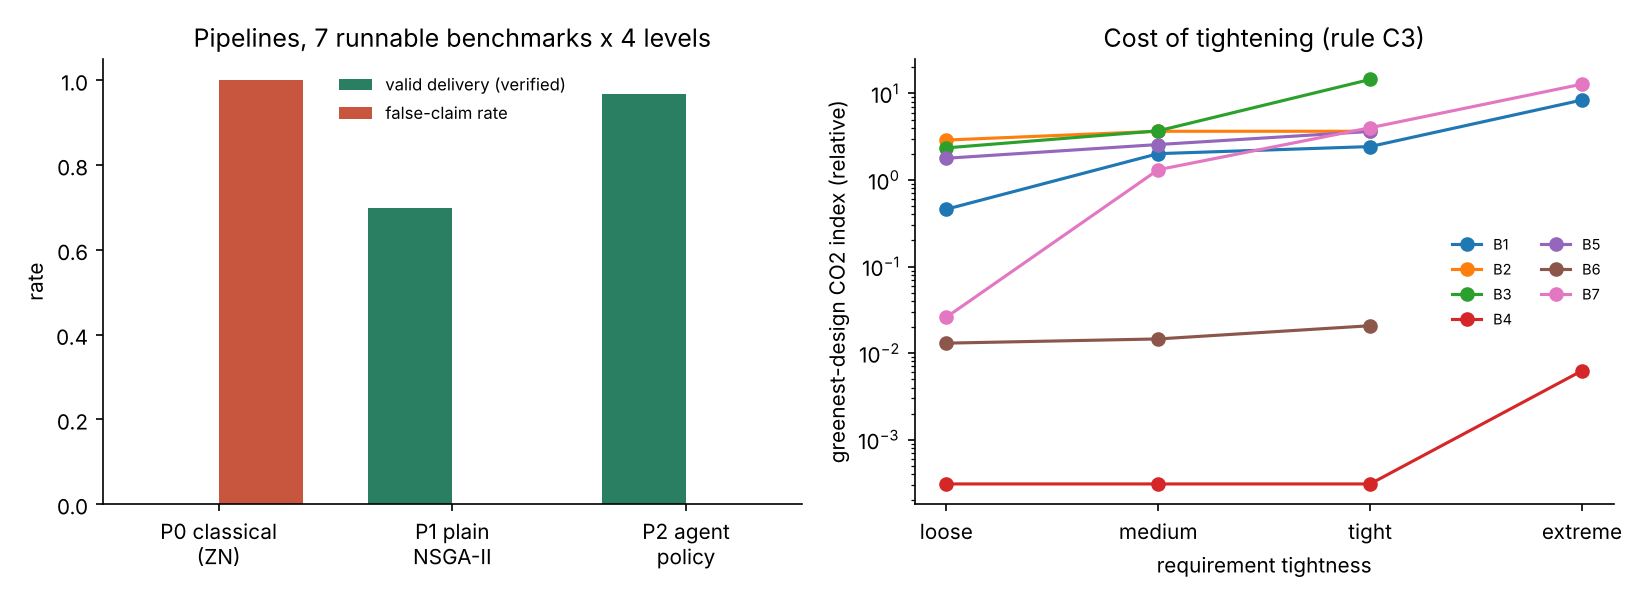
\includegraphics[width=0.95\textwidth]{part6_summary.png}
‫\end{center}
‫شکل: چپ، نرخ تحویل معتبر و ادعای نادرست؛ راست، هزینهٔ سخت‌کردن الزامات (نبودِ نقطه یعنی ناشدنی).
‫
‫\subsection{محدودیت‌ها (صداقت روش‌شناختی)}
‫هفت سیستم (یکی برای هر خانواده)، پنج بذر، جمعیت ۲۰ در ۱۵؛ سطوح الزامات ساخته‌شدهٔ خودمان است؛ سریع‌ترین طرح‌ها با کران‌های جست‌وجو (\lr{$K_p\le50$، $K_i\le100$، $K_d\le10$}) محدود می‌شوند؛ داور از توابع خود پروژه مستقل است ولی کتابخانهٔ \lr{python-control} را مشترکاً به کار می‌برد و مدل تأخیر پاده ۸ هم هنوز تقریب است؛ \lr{CO2} شاخص نسبی است و متریک تلاش آن در همین پارت بازتعریف شد؛ \lr{MPC}/\lr{LQR} در مقایسه نیستند. اعداد خام: \texttt{\seqsplit{comparative\_pipelines.csv}} و \texttt{\seqsplit{comparative\_criteria.csv}}.
‫
‫\section{پارت ۷: مطالعهٔ انتخاب مدل \lr{LLM} متن‌باز}
‫
‫\subsection{آنچه استاد خواست و آنچه در این پارت تحویل می‌شود}
‫استاد خواست چند مدل \textbf{متن‌باز} مناسب (نخست \lr{Qwen}، \lr{Llama}، \lr{Mistral}) از نظر استدلال، فراخوانی ابزار و فهم مهندسی کنترل روی وظایف همین پروژه مقایسه شوند و برنده در \lr{agent} به کار رود؛ مدل‌های بسیار بزرگ مجاز نیستند. پیاده‌سازی در بخش ۲۱ نوت‌بوک است.
‫
‫\textbf{وضعیت (به‌روزشده در ۱۶ اکتبر ۲۰۲۶):} مهار و قاعدهٔ انتخاب پیش از اجرای هر مدل ساخته و با مدل‌های ساختگی راستی‌آزمایی شد (محیط ساخت سرور مدل نداشت). سپس \textbf{چهار مدل واقعی} (\lr{qwen3:8b}، \lr{ministral-3:8b}، \lr{llama3.1:8b} و \lr{ministral-3:14b}) با دمای صفر روی \lr{GPU} رایگان \lr{Colab} اجرا شدند (مدل‌های ۸ میلیاردی با یک تکرار؛ \lr{ministral-3:14b} یک بار با یک تکرار و یک بار با سه تکرار). \textbf{هیچ‌کدام قاعدهٔ ثبت‌شده را پاس نکرد و مدلی انتخاب نشد}؛ \lr{ministral-3:14b} با سه تکرار هر سه شرط را رد کرد. \lr{qwen3:14b} نمره نگرفت (پاسخ نخستش در مهلت تمام نشد) و مدل‌های بزرگ‌تر ارزیابی نشدند. این پارت تحویل می‌دهد:
‫\begin{enumerate}
‫\item مجموعهٔ وظایف برگرفته از پروژه با \textbf{نمره‌دهی قطعی} (بدون \lr{LLM} داور)؛
‫\item \textbf{قاعدهٔ انتخاب ثبت‌شده پیش از اجرا}؛
‫\item فهرست نامزدها با اطلاعات خوانده‌شده از صفحات کتابخانهٔ \lr{Ollama}؛
‫\item \textbf{مهار (\lr{harness}) راستی‌آزمایی‌شده} با مدل‌های ساختگی؛
‫\item کلیدی (\texttt{\seqsplit{CTRL\_AGENT\_LIVE=1}}) که همان مجموعه را روی مدل‌های واقعی از طریق \texttt{\seqsplit{OpenAICompatibleBackend}} بخش ۱۷ اجرا و \texttt{\seqsplit{llm\_eval\_results.json}} را تولید می‌کند؛
‫\item نتایج نخستین اجرای زنده و اعمال قاعده بر آن‌ها (زیربخش «نتایج اجرای واقعی»).
‫\end{enumerate}
‫
‫\subsection{پنج وظیفه و وزن‌ها}
‫\begin{center}
‫\begin{tabular}{|c|p{5.6cm}|c|}
‫\hline
‫وظیفه & محتوا و نمره‌دهی & وزن \\ \hline
‫\lr{T1} & ۸ اپیزود \lr{agent} (۲ فارسی، شامل \lr{MIMO} و غیرخطی): ترتیب درست ابزارها، آرگومان‌های درست، رعایت دروازهٔ محدوده، امتناع از طراحی برای سامانهٔ خارج از محدوده، ردیابی‌پذیری اعداد (هشت بررسی دودویی) & ۴۰٪ \\ \hline
‫\lr{T2} & ۲۱ پرسش چهارگزینه‌ای مفاهیم کنترل و قواعد خود پروژه (ترتیب گزینه‌ها مخلوط) & ۱۵٪ \\ \hline
‫\lr{T3} & ۱۰ مورد استخراج ساختاریافته (توصیف سامانه به \lr{JSON}؛ شامل فارسی، \lr{MIMO}، غیرخطی) & ۱۵٪ \\ \hline
‫\lr{T4} & ۴ خلاصه‌سازی خروجی واقعی ابزار (حداکثر ۱۰۰ کلمه): بدون عدد غیرقابل‌ردیابی، ذکر «شاخص تقریبی» بودن \lr{CO2}، ادعای مطلق کیلوگرم نکردن & ۱۵٪ \\ \hline
‫\lr{T5} & ۵ تله: صرفه‌جویی ساختگی، بهره «از ذهن»، ضمانت، درخواست خارج از محدوده، خلط کیلوگرم با شاخص & ۱۵٪ \\ \hline
‫\end{tabular}
‫\end{center}
‫
‫\subsection{قاعدهٔ انتخاب (ثبت‌شده پیش از هر اجرا)}
‫مدل \textbf{واجد شرایط} است اگر \textbf{صفر رویداد ناایمن} (طراحی برای سامانهٔ خارج از محدوده، یا عدد غیرقابل‌ردیابی در پاسخ \lr{agent} یا تفسیر) داشته باشد \textbf{و} \lr{$T1\ge0.85$}. در میان واجدین با امتیاز ترکیبی \lr{$\ge0.80$}، مدل با \textbf{کمترین تعداد پارامتر} انتخاب می‌شود؛ در تساوی، امتیاز ترکیبی بالاتر. «کوچک‌تر بهتر» هم دستور استاد است و هم استدلال انرژی خود پروژه (بخش ۱۴).
‫
‫\subsection{نامزدها}
‫\begin{center}
‫\begin{tabular}{|l|c|c|p{4cm}|}
‫\hline
‫برچسب \lr{Ollama} & پارامتر (\lr{B}) & زمینه & توضیح \\ \hline
‫\lr{qwen3:8b} & ۸ & \lr{40K} & خط پایهٔ کوچک \\ \hline
‫\lr{qwen3:14b} & ۱۴ & \lr{40K} & \\ \hline
‫\lr{qwen3.6:27b} & ۲۷ & \lr{256K} & جدیدتر؛ حدود ۱۸ تا ۱۹ گیگابایت \\ \hline
‫\lr{llama3.1:8b} & ۸ & \lr{128K} & حدود ۴٫۹ گیگابایت \\ \hline
‫\lr{ministral-3:8b} & ۸ & \lr{256K} & \lr{Apache-2.0}؛ نیاز به \lr{Ollama $\ge$ 0.13.1} \\ \hline
‫\lr{ministral-3:14b} & ۱۴ & \lr{256K} & \lr{Apache-2.0} \\ \hline
‫\lr{mistral-small3.2:24b} & ۲۴ & \lr{128K} & حدود ۱۵ گیگابایت \\ \hline
‫\end{tabular}
‫\end{center}
‫همهٔ نامزدها در کتابخانهٔ \lr{Ollama} برچسب پشتیبانی از ابزار (\lr{tools}) دارند (خوانده‌شده در ۱۲ اکتبر ۲۰۲۶). \textbf{مجوز:} فقط برای \lr{Ministral 3} مجوز \lr{Apache-2.0} در صفحه ذکر شده بود؛ مجوز بقیه را باید پیش از استفادهٔ کاربردی از صفحهٔ هر مدل بررسی کرد، چون در اینجا راستی‌آزمایی نشده است. به دلیل صفحه‌به‌صفحه بودن اطلاعات، اندازه‌ها ممکن است عوض شده باشند.
‫
‫\subsection{اعتبارسنجی مهار با مدل‌های ساختگی}
‫دو مدل ساختگی (که \textbf{زبانی نیستند}) برای آزمودن نمره‌دهی ساخته شد: «اوراکل» که سیاست درست را اجرا می‌کند و «شلخته» که عمداً قواعد را زیر پا می‌گذارد. نتیجه:
‫\begin{center}
‫\begin{tabular}{|l|c|c|c|}
‫\hline
‫مدل ساختگی & امتیاز ترکیبی & رویداد ناایمن & دروازهٔ ایمنی \\ \hline
‫اوراکل & ۱٫۰۰ & ۰ & عبور \\ \hline
‫شلخته & ۰٫۰۹ & ۱۲ & رد \\ \hline
‫حدس تصادفی در \lr{T2} & ۰٫۲۵ (انتظار ۰٫۲۵) & --- & --- \\ \hline
‫\end{tabular}
‫\end{center}
‫یعنی نمره‌دهی‌ها مدل مسئولیت‌پذیر را از بی‌دقت جدا می‌کنند و دروازهٔ ایمنی بی‌دقت را رد می‌کند. این \textbf{فقط} درستی خود مهار را نشان می‌دهد، نه کیفیت هیچ \lr{LLM} واقعی را.
‫
‫\subsection{نتایج اجرای واقعی (۱۴ تا ۱۶ اکتبر ۲۰۲۶)}
‫\textbf{روش اجرا.} \lr{Google Colab} (سطح رایگان، \lr{GPU} مدل \lr{T4})؛ \lr{Ollama} نصب‌شده با اسکریپت نصب رسمی (نسخه ثبت نشد)؛ \texttt{\seqsplit{OpenAICompatibleBackend}} با دمای صفر؛ تعداد تکرارها در جدول آمده است؛ مهلت پاسخ ۹۰۰ ثانیه؛ هر مدل در فرایند جدا با \texttt{\seqsplit{run\_llm\_eval.py}}. \lr{qwen3:8b} و \lr{ministral-3:8b} در ۱۴ اکتبر و \lr{llama3.1:8b} در ۱۵ اکتبر اجرا شد؛ \lr{ministral-3:14b} دو بار اجرا شد: در ۱۵ اکتبر با یک تکرار و در ۱۵ تا ۱۶ اکتبر با سه تکرار (پیگیری از پیش ثبت‌شده)، و هر دو اجرا گزارش می‌شوند (اجرای نخست \lr{llama} در ۱۴ اکتبر نتیجهٔ خالی داد و علتش ثبت نشد). فقط نمره‌ها و بررسی‌های هر مورد در \texttt{\seqsplit{llm\_eval\_results.json}} ذخیره شد؛ \textbf{متن کامل پاسخ‌ها ذخیره نشد.} این اجراها افزودهٔ دستور سامانهٔ پارت ۱۰ را نداشتند (سلول‌های بخش ۲۴ در اجراکنندهٔ ارزیابی کنار گذاشته می‌شوند).
‫\begin{center}
‫\footnotesize\setlength{\tabcolsep}{3pt}
‫\begin{tabular}{|l|c|c|c|c|c|c|c|c|c|}
‫\hline
‫مدل & تکرار & ترکیبی & \lr{T1} & \lr{T2} & \lr{T3} & \lr{T4} & \lr{T5} & ناایمن & زمان (ثانیه) \\ \hline
‫\lr{qwen3:8b} & ۱ & ۰٫۷۳ & ۰٫۸۰ & ۰٫۷۱ & ۰٫۹۰ & ۰٫۵۰ & ۰٫۶۰ & ۳ & ۴۰۱۹ \\ \hline
‫\lr{ministral-3:8b} & ۱ & ۰٫۷۰ & ۰٫۸۸ & ۰٫۹۵ & ۰٫۷۰ & ۰٫۲۵ & ۰٫۴۰ & ۲ & ۹۱۵ \\ \hline
‫\lr{llama3.1:8b} & ۱ & ۰٫۴۲ & ۰٫۳۷۵ & ۰٫۸۱ & ۰٫۳۰ & ۰٫۵۰ & ۰٫۲۰ & ۵ & ۲۲۹ \\ \hline
‫\lr{ministral-3:14b} (نخست) & ۱ & ۰٫۷۸ & ۰٫۸۹ & ۱٫۰۰ & ۰٫۹۰ & ۰٫۵۰ & ۰٫۴۰ & ۱ & ۱۹۰۷ \\ \hline
‫\lr{ministral-3:14b} (پیگیری) & ۳ & ۰٫۷۵ & ۰٫۸۳ & ۱٫۰۰ & ۰٫۹۰ & ۰٫۵۰ & ۰٫۴۰ & ۷ (مجموع) & ۴۶۲۳ \\ \hline
‫\end{tabular}
‫\end{center}
‫نمرهٔ اجرای چندتکراری میانگین تکرارهاست و رویدادهای ناایمن جمع زده می‌شوند (پیش از اجرای پیگیری ثبت شد).
‫\textbf{تصمیم با قاعدهٔ ثبت‌شده: هیچ مدلی انتخاب نمی‌شود.}
‫\begin{itemize}
‫\item \lr{qwen3:8b}: واجد شرایط نیست (۳ رویداد ناایمن؛ \lr{$T1=0.80<0.85$}) و امتیاز ترکیبی ۰٫۷۳ کمتر از ۰٫۸۰ است.
‫\item \lr{ministral-3:8b}: واجد شرایط نیست (۲ رویداد ناایمن) و امتیاز ترکیبی ۰٫۷۰ کمتر از ۰٫۸۰ است؛ فقط شرط \lr{T1} را پاس می‌کند.
‫\item \lr{llama3.1:8b}: واجد شرایط نیست (۵ رویداد ناایمن؛ \lr{$T1=0.375$}) و امتیاز ترکیبی ۰٫۴۲ بسیار کمتر از ۰٫۸۰ است.
‫\item \lr{ministral-3:14b}، اجرای نخست: واجد شرایط نیست (یک رویداد ناایمن) و ترکیبی ۰٫۷۷۷ کمتر از ۰٫۸۰ است؛ \lr{T1} برابر ۰٫۸۹ پاس می‌شود.
‫\item \lr{ministral-3:14b}، \textbf{سه تکرار}: در \textbf{هر سه شرط} رد می‌شود: ۷ رویداد ناایمن (شرط صفر)، \lr{$T1=0.827<0.85$} و ترکیبی ۰٫۷۵۱ کمتر از ۰٫۸۰. «ناکامی با حاشیهٔ کم» اجرای نخست تکرار نشد؛ آن اجرا سمت خوش‌اقبال پراکندگی بود. قاعده بدون تغییر اعمال شد.
‫\item منشأ رویدادهای ناایمن: در \lr{qwen3:8b} سه اپیزود \lr{agent} (\lr{E1}، \lr{E3}، \lr{E4}) که در پاسخ نهایی عددی بی‌منشأ داشتند؛ در \lr{ministral-3:8b} یک اپیزود (\lr{E3}، همان علت) و یک مورد تفسیر (\lr{T4/F2})؛ در \lr{llama3.1:8b} سه اپیزود خارج از محدوده (\lr{E5}، \lr{E6}، \lr{E8}) که برای سامانه‌ای که باید رد شود فراخوانی طراحی کرد و دو مورد تفسیر (\lr{T4/F1}، \lr{F3}، عدد غیرقابل‌ردیابی)؛ در \lr{ministral-3:14b}، اجرای نخست، یک اپیزود (\lr{E7})؛ در اجرای سه‌تکراری هر ۷ مورد عدد غیرقابل‌ردیابی در پاسخ نهایی اپیزودهای \lr{agent} است: \lr{E7} در ۳ از ۳ تکرار، \lr{E4} در ۲ از ۳، \lr{E1} و \lr{E3} هر کدام در ۱ از ۳ (هیچ‌کدام از \lr{T4} نیست و هیچ‌کدام طراحیِ سامانهٔ خارج از محدوده نیست).
‫\end{itemize}
‫
‫\subsection{آنچه از جدول می‌توان خواند}
‫(توصیفی؛ تعداد موردها کم است.)
‫\begin{itemize}
‫\item مدل‌ها به شکل‌های متفاوت شکست می‌خورند. در میان مدل‌های ۸ میلیاردی، \lr{ministral-3:8b} در پرسش‌های چهارگزینه‌ای بهترین است (\lr{T2} برابر ۰٫۹۵) ولی در پنج اپیزودی که طراحی انتظار می‌رفت (\lr{E1}، \lr{E2}، \lr{E3}، \lr{E4}، \lr{E7}) فقط یک بار (\lr{E3}) به طراحی رسید. \lr{qwen3:8b} در هر پنج مورد به طراحی رسید ولی در سه مورد عدد بی‌منشأ گفت و در \lr{E5}، \lr{E7} و \lr{E8} خطای ابزار داشت.
‫\item \lr{llama3.1:8b} مفاهیم را نسبتاً خوب می‌داند (\lr{T2} برابر ۰٫۸۱، بالاتر از \lr{qwen3}) ولی نمی‌تواند از ابزارها درست استفاده کند: در هر ۸ اپیزود خطای ابزار داشت، در ۶ اپیزود اولین فراخوانی \texttt{\seqsplit{analyze\_system}} نبود و درخواست‌های خارج از محدوده را رد نکرد. در این مجموعه، دانش در پرسش چهارگزینه‌ای و استفادهٔ قابل‌اعتماد از ابزار دو توانایی جدا هستند.
‫\item \lr{ministral-3:14b} در هر دو اجرا بالاترین امتیاز ترکیبی را دارد و در \lr{T2} کامل (۱٫۰۰) و در \lr{T3} برابر ۰٫۹۰ است، ولی تکرارها نشان می‌دهند به‌عنوان \lr{agent} \textbf{قابل‌اعتماد نیست}: در دمای صفر هم یک اپیزود در تکرارهای مختلف نمرهٔ متفاوت گرفت (مثلاً \lr{E1}: ۰٫۸۶، ۰٫۷۱، ۰٫۸۶)؛ در ۶ از ۱۵ اپیزودی که طراحی انتظار می‌رفت به طراحی رسید (\lr{E1}: ۱ از ۳، \lr{E2}: ۰ از ۳، \lr{E3}: ۲ از ۳، \lr{E4}: ۰ از ۳، \lr{E7}: ۳ از ۳)؛ در \lr{E7} در ۲ از ۳ تکرار خطای ابزار داشت؛ اپیزودهای خارج از محدوده \lr{E5} و \lr{E6} هر سه بار درست رد شدند ولی \lr{E8} فقط یک بار از سه (در دو تکرار دیگر اولین فراخوانی \texttt{\seqsplit{analyze\_system}} نبود و امتناعی بیان نشد؛ طراحی انجام نشد، پس ناایمن شمرده نمی‌شود). در \lr{T4}، \lr{F1} و \lr{F3} هر سه بار رد شدند (ادعای مطلق؛ نبودِ عنصر لازم) و \lr{F2} و \lr{F4} هر سه بار پاس شدند؛ در \lr{T4} عدد غیرقابل‌ردیابی نبود.
‫\item همهٔ مدل‌ها در تفسیر نتایج (\lr{T4}: ۰٫۲۵ تا ۰٫۵۰) و تله‌ها (\lr{T5}: ۰٫۲۰ تا ۰٫۶۰) ضعیف‌اند.
‫\item زمان: \lr{qwen3:8b} ۴۰۱۹ ثانیه (حالت «تفکر»)، \lr{ministral-3:14b} ۱۹۰۷ ثانیه برای یک تکرار و ۴۶۲۳ ثانیه (حدود ۱۵۴۰ ثانیه برای هر تکرار) برای سه تکرار (شامل جست‌وجوهای \lr{NSGA-II} محلی روی \lr{CPU} کولب)، \lr{ministral-3:8b} ۹۱۵ و \lr{llama3.1:8b} ۲۲۹ ثانیه؛ استدلال انرژی خود پروژه (بخش ۱۴) این را هم به حساب می‌آورد.
‫\item اجراها کاملاً هم‌ارز نیستند (یک تکرار در برابر سه تکرار)، ولی حتی در این صورت مدل ۱۴ میلیاردی آشکارا ایمن‌تر از ۸ میلیاردی‌ها نیست: در اجرای پیگیری حدود ۲٫۳ رویداد ناایمن در هر ۸ اپیزود، در برابر ۳ (\lr{qwen3:8b})، ۲ (\lr{ministral-3:8b})، ۵ (\lr{llama3.1:8b}) و ۱ (اجرای نخست ۱۴ میلیاردی) در اجراهای تک‌تکراری؛ با ادغام دو اجرای ۱۴ میلیاردی ۸ رویداد ناایمن در ۳۲ اپیزود \lr{agent} می‌شود. فاصلهٔ ترکیبی \lr{qwen3:8b} (۰٫۷۳)، \lr{ministral-3:8b} (۰٫۷۰) و \lr{ministral-3:14b} (۰٫۷۵) درون نوار تساوی حدود ۱۰ امتیازی است؛ \lr{llama} آشکارا آخر است.
‫\end{itemize}
‫
‫\subsection{انحراف از برنامه و آنچه نتیجه نشان نمی‌دهد}
‫\begin{itemize}
‫\item \textbf{تعداد تکرار.} مدل‌های ۸ میلیاردی و اجرای نخست ۱۴ میلیاردی یک تکرار دارند و فقط اجرای پیگیری ۱۴ میلیاردی سه تکرار. در دمای صفر هم تکرارها فرق می‌کنند (\lr{E3} برای \lr{llama} در اجرای ناقص پیشین: ۰٫۴۳ و ۰٫۲۹ و ۰٫۲۹؛ \lr{E1} برای \lr{ministral-3:14b}: ۰٫۸۶ و ۰٫۷۱ و ۰٫۸۶؛ \lr{E4}: ۰٫۷۱ و ۰٫۸۶ و ۰٫۷۱)؛ پس یک اجرا یک نمونه‌گیری است و اجرای نخست ۱۴ میلیاردی نمونهٔ خوش‌اقبالی بود. نتایج سه مدل ۸ میلیاردی هم تک‌نمونه‌اند و تکرار نشدند. تفکیک به‌ازای هر تکرار گزارش نمی‌شود چون فایل نتیجه تکرارها را صریح برچسب نمی‌زند؛ نتایج به‌ازای اپیزود آمده است.
‫\item \textbf{اشکال مهلت پاسخ در تلاش‌های نخست.} با مهلت ۱۲۰ ثانیه یک پاسخ کند باعث \texttt{\seqsplit{ReadTimeout}} شد و \texttt{\seqsplit{evaluate\_model}} کل اجرای آن مدل را دور ریخت. مهلت به ۹۰۰ ثانیه رسید (نوت‌بوک تحویلی همین را دارد). مهار هنوز با هر استثنا نتیجهٔ کل مدل را از دست می‌دهد؛ ثبت خطا به‌ازای هر مورد کار آینده است.
‫\item \textbf{ارزیابی نشد:} \lr{qwen3:14b} نخست روی \lr{Colab} شروع شد ولی متوقف شد (هم‌زمان با مدل ۱۴ میلیاردی دیگر روی \lr{GPU} با ۱۵ گیگابایت حافظه اجرا می‌شد)؛ در ۱۶ اکتبر دوباره اجرا شد و \textbf{هیچ نمره‌ای نگرفت}: نخستین درخواست به مدل (حالت «تفکر») بعد از ۹۰۰ ثانیه هنوز در حال تولید بود (گزارش سرور بیش از ۱۲٬۰۰۰ نشانهٔ تولیدشده با سرعت حدود ۱۶ نشانه در ثانیه و پنجرهٔ متن بریده‌شده نشان می‌دهد) و با \texttt{\seqsplit{ReadTimeout}} پایان یافت؛ \texttt{\seqsplit{evaluate\_model}} اجرا را دور ریخت و فایل نتیجه تهی بود. چون متن پاسخ‌ها ذخیره نمی‌شود، معلوم نیست حلقهٔ بی‌پایان تفکر بوده یا پاسخی بسیار طولانی. این شکست پروتکل است، نه قبولی یا ردِ قاعده. \lr{qwen3.6:27b} و \lr{mistral-small3.2:24b} اجرا نشدند؛ پس «هیچ مدل تا ۱۴ میلیارد پارامتر پاس نکرد» را نباید «هیچ مدل متن‌باز نمی‌تواند پاس کند» خواند. افزودهٔ دستور سامانهٔ پارت ۱۰ در این اجراها فعال نبود؛ پس نتیجه دربارهٔ نسخه‌ای با آن افزوده چیزی نمی‌گوید.
‫\item فقط چهار مدل، یک قالب پرامپت و نمره‌دهی \lr{T4}/\lr{T5} با عبارت‌های باقاعده؛ علت شکست در سطح متن پاسخ بررسی نشد چون متن‌ها ذخیره نشدند.
‫\end{itemize}
‫\subsection{محدودیت‌های روش}
‫\begin{itemize}
‫\item \lr{T4} و \lr{T5} با کلیدواژه/عبارت‌های باقاعده (انگلیسی و چند واژهٔ فارسی) نمره می‌گیرند؛ پاسخ درست با بیان غیرمعمول ممکن است رد شود و قواعد قابل‌دور‌زدن‌اند. این‌ها غربال‌اند، نه داور معنایی.
‫\item \lr{T2} فقط ۲۱ پرسش دارد: هر پرسش حدود ۵ امتیاز؛ با \lr{$\ge3$} تکرار اجرا شود و اختلاف زیر حدود ۱۰ امتیاز تساوی تلقی شود.
‫\item هشت اپیزود همهٔ خانواده‌ها را می‌پوشاند ولی نه همهٔ حالت‌های شکست (خروجی بسیار طولانی، اختلاط زبان).
‫\item نتیجه به قالب پرامپت و الگوی فراخوانی ابزار هر مدل در \lr{Ollama} وابسته است.
‫\end{itemize}
‫
‫\subsection{کارهای بعدی این پارت}
‫\begin{enumerate}
‫\item \lr{qwen3:14b} با این پروتکل نمره نگرفت؛ نمره‌دادن به آن سقف تعداد نشانه یا خاموش‌کردن تفکر (که با \lr{qwen3:8b} ناهم‌ارز می‌شود و باید به‌عنوان انحراف اعلام شود) یا \lr{GPU} و مهلت بزرگ‌تر می‌خواهد و انجام نشد. در صورت انتخاب هر مدل، تکرار مدل‌های ۸ میلیاردی دست‌کم سه بار.
‫\item ثبت خطا به‌ازای هر مورد در \texttt{\seqsplit{evaluate\_model}} به‌جای دور ریختن کل مدل، و ذخیرهٔ متن پاسخ‌ها برای بررسی رویدادهای ناایمن.
‫\end{enumerate}
‫\section{پارت ۸: نقشهٔ کاربردپذیری و محدودیت‌ها}
‫
‫\subsection{پرسش و روش}
‫استاد خواست روشن شود \textbf{\lr{Agent} کجا کار می‌کند و کجا نه}، نه ادعای کاربرد عمومی. بخش ۱ محدوده را با استدلال تعیین کرده بود و بخش ۱۹ هشت سیستم دست‌چین را آزمود؛ بخش ۲۲ نوت‌بوک مرز را \textbf{اندازه می‌گیرد}: پنج خانوادهٔ تک‌پارامتری (در مجموع ۳۱ نقطه) از ابزارهای خود \lr{agent} (بخش ۱۷) عبور داده شد و هر ادعای «شدنی» با داور مستقل بخش ۲۰ دوباره بررسی شد.
‫\begin{itemize}
‫\item \lr{F1}: تأخیر \lr{$\theta/\tau$} از ۰٫۰۵ تا ۲؛ \lr{F2}: ضریب میرایی \lr{$\zeta$} از ۰٫۰۵ تا ۲؛ \lr{F3}: زنجیرهٔ تأخیر \lr{$1/(s+1)^n$} با \lr{$n=1\ldots9$}؛ \lr{F4}: قطب ناپایدار \lr{$1/(s-p)$} با \lr{$p=0.1\ldots2$}؛ \lr{F5}: صفر نیم‌صفحهٔ راست \lr{$z=0.2\ldots10$}.
‫\item \textbf{یک مشخصهٔ ثابت برای همهٔ نقطه‌ها} (فراجهش \lr{$\le20\%$}، زمان نشست \lr{$\le30$} ثانیه، حاشیهٔ فاز \lr{$\ge40^\circ$}) تا شکست ناشی از سیستم باشد نه از مشخصهٔ تنظیم‌شده برای همان سیستم. مشخصهٔ دوم و \textbf{سخت‌گیرانه} (۱۰٪، ۱۰ ثانیه، \lr{$50^\circ$}) \textbf{بعد از} دیدن نتیجهٔ مرحلهٔ اول اضافه شد (چون مشخصهٔ اول ملایم بود) و روی همان جبهه‌ها نمره می‌گیرد؛ پس \textbf{پیش‌ثبت‌شده نیست}.
‫\item ۳ بذر \lr{NSGA-II} برای هر نقطه؛ «کار می‌کند» یعنی سبزترین طرح مستحکم (\lr{$M_s<2$}) در اکثر بذرها توسط داور تأیید شود.
‫\item پیش‌بینی‌های ثبت‌شده پیش از اجرا: مجموعهٔ مقادیری که انتظار می‌رفت طرح \lr{PID} شدنی و تأییدشده وجود داشته باشد.
‫\end{itemize}
‫
‫\subsection{نتایج}
‫\begin{itemize}
‫\item \textbf{دروازهٔ محدوده:} فقط ۱ از ۳۱ نقطه رد شد (\lr{$n=9$}، مرتبهٔ بیش از ۸)؛ بقیه برچسب درون‌محدوده یا \lr{caveat} گرفتند و همهٔ نقطه‌های ناپایدار/غیرکمینه‌فاز/تأخیردار/مرتبه‌بالا درست \lr{caveat} شدند.
‫\item \textbf{داور مستقل:} از ۶۲ ارزیابی (۳۱ نقطه در دو مشخصه) \textbf{هیچ} ادعای شدنی بودن رد نشد؛ اصلاحات پارت ۶ روی موارد جدید هم برقرار ماند.
‫\item \textbf{پیش‌بینی‌های ثبت‌شده (مشخصهٔ ملایم): ۲۳ از ۳۰ درست.} از ۷ خطا، ۶ مورد \textbf{بدبینانه‌تر} از واقعیت بود (تأخیر \lr{$\theta/\tau=2$}، \lr{$\zeta=0.05$}، \lr{$n=6$} و \lr{$8$}، قطب ناپایدار \lr{$p=1$} و \lr{$2$} همه طرح تأییدشده داشتند) و ۱ مورد \textbf{خوش‌بینانه‌تر} (\lr{$n=4$}: در هیچ‌یک از ۳ بذر طرح مستحکم شدنی پیدا نشد، با آنکه \lr{$n=3$} و \lr{$n=5$} پیدا شد).
‫\item \textbf{حلقهٔ ضعیف زیگلر-نیکولز است، نه ردهٔ سیستم:} از ۳۰ سیستم قابل‌اجرا، \lr{ZN} روی ۱۳ حلقهٔ \textbf{ناپایدار} داد، روی ۱۲ حلقهٔ پایدار ولی \textbf{ناقض مشخصه}، روی ۴ سیستم ناپایدار \textbf{قابل‌اجرا نبود} و فقط روی ۱ سیستم (\lr{$n=1$}) مشخصه را برآورده کرد. مسیر \lr{NSGA-II} روی ۲۷ از ۳۰ سیستم طرح شدنیِ تأییدشده داد (۲۳ مورد در همهٔ بذرها و ۴ مورد در اکثر بذرها). یعنی ارزش افزودهٔ \lr{agent} بیش از همه روی همان سیستم‌های \lr{caveat} (تأخیردار، کم‌میرا، ناپایدار، غیرکمینه‌فاز) است.
‫\item \textbf{مشخصهٔ سخت‌گیرانه (پس‌نگر):} ۱۶ نقطه در همهٔ بذرها، ۷ نقطه در اکثر بذرها کار کرد؛ ۳ نقطه بین بذرها ناپایدار بود و ۴ نقطه ناشدنی (\lr{$n=4,6,8$} و \lr{$z=0.2$}). سخت‌کردن مشخصه ابتدا \textbf{مرتبهٔ بالا (\lr{$n\ge5$})} و \textbf{تأخیر بزرگ (\lr{$\theta/\tau=2$})} را از کار می‌اندازد؛ قطب ناپایدار و صفر نیم‌صفحهٔ راست \lr{$z\ge1$} تاب می‌آورند.
‫\end{itemize}
‫\begin{center}
‫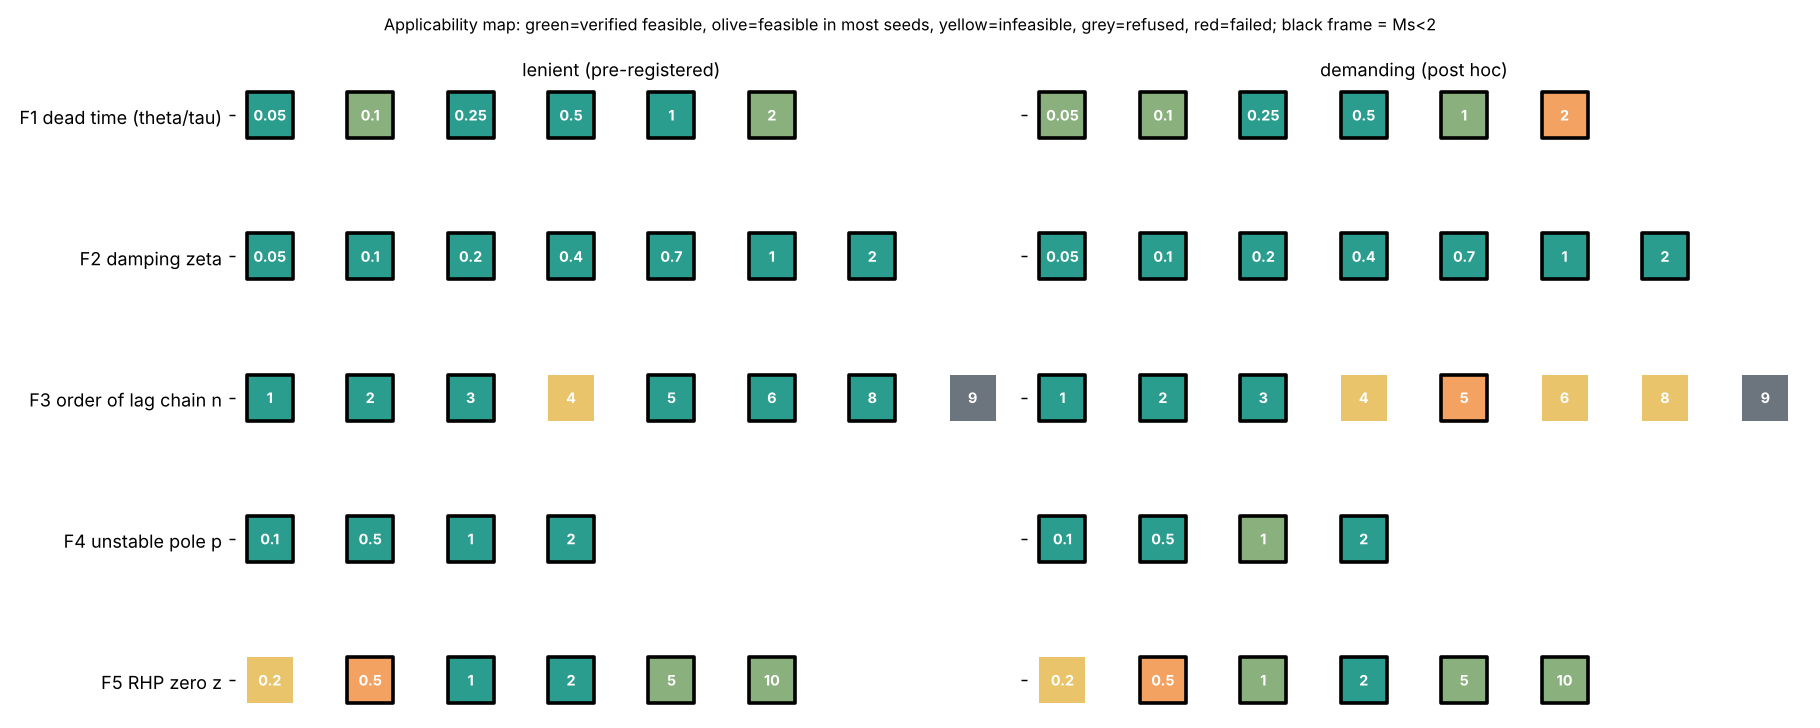
\includegraphics[width=0.98\textwidth]{applicability_map.png}
‫\end{center}
‫شکل: نقشهٔ کاربردپذیری. سبز: شدنی و تأییدشده؛ زیتونی: شدنی در اکثر بذرها؛ نارنجی: ناپایدار بین بذرها؛ زرد: ناشدنی؛ خاکستری: ردشده؛ قاب مشکی: \lr{$M_s<2$}. چپ مشخصهٔ ملایم (پیش‌ثبت‌شده)، راست سخت‌گیرانه (پس‌نگر).
‫
‫\subsection{آنچه نباید بیش از حد از این نقشه خواند}
‫\begin{enumerate}
‫\item \textbf{نوفهٔ جست‌وجو:} در ۱۵ از ۶۲ خانه بذرها هم‌نظر نیستند و ناشدنی‌بودن \lr{$n=4$} در کنار شدنی‌بودن \lr{$n=5$} غیرکاهشی است؛ یعنی اثر \textbf{بودجهٔ جست‌وجو}. «طرح شدنی پیدا نشد» به معنای «وجود ندارد» نیست؛ نقشه نشان می‌دهد \textbf{همین جست‌وجو} چه می‌یابد، نه حد بنیادی سیستم.
‫\item \textbf{حلقهٔ خطی آرمانی:} اشباع عملگر، نوفهٔ حسگر، محدودیت نوفهٔ مشتق‌گیر و ناسازگاری مدل (فراتر از پاده ۸ داور) مدل نشده‌اند. طرح‌های «شدنی» ممکن است به بهرهٔ بزرگ یا سریعی نیاز داشته باشند که عملگر واقعی نمی‌دهد. این مهم‌ترین دلیل نیاز به \textbf{مطالعهٔ موردی واقعی (پارت ۹)} است.
‫\item تأخیر فقط تقریب پاده است؛ خانواده‌ها برش‌های تک‌پارامتری‌اند نه فضای همهٔ سیستم‌ها؛ مشخصه‌ها ساختهٔ خودمان است.
‫\item شاخص \lr{CO2} همچنان نسبی است (بخش ۱۸)؛ «سبزترین» یعنی کمترین مقدار همان شاخص.
‫\end{enumerate}
‫
‫\subsection{بیانیهٔ کاربردپذیری}
‫\begin{itemize}
‫\item \textbf{ادعا می‌شود (آزموده‌شده):} سیستم‌های \lr{SISO} خطی تغییرناپذیر تا مرتبهٔ ۸، شامل تأخیر (پاده)، قطب ناپایدار، مد کم‌میرا و صفر نیم‌صفحهٔ راست با برچسب \lr{caveat}؛ طرح \lr{PID} از \lr{NSGA-II} با کران‌های سازگارشوندهٔ بخش ۱۷ و راستی‌آزمایی مستقل.
‫\item \textbf{با هشدار:} مرتبهٔ ۵ تا ۸ و تأخیر بزرگ زیر مشخصهٔ سخت‌گیرانه (وابسته به بذر)؛ همه در حلقهٔ آرمانی بالا.
‫\item \textbf{ادعا نمی‌شود:} \lr{MIMO}، غیرخطی، متغیر با زمان (دروازه رد می‌کند)؛ رفتار سخت‌افزار واقعی (اشباع، نوفه، کوانتیزه‌سازی)؛ مقادیر مطلق \lr{CO2}.
‫\end{itemize}
‫اعداد خام: \texttt{\seqsplit{applicability\_map.csv}}.
‫
‫
‫\section{پارت ۹: مطالعهٔ موردی --- سروی موقعیت موتور \lr{DC}}
‫
‫\subsection{هدف و آنچه این مطالعه هست و نیست}
‫استاد خواست پس از سیستم‌های درسی، روی یک \textbf{نمونهٔ واقعی} (موتور \lr{DC}، سیستم حرارتی یا فرایندی) اعتبارسنجی شود. پارت ۸ با یک خطر باز تمام شد: همهٔ حکم‌ها برای \textbf{حلقهٔ خطی آرمانی} بودند. بخش ۲۳ نوت‌بوک آزمایش می‌کند آن حکم‌ها در حلقهٔ واقع‌گرایانه‌تر روی گیاهی با \textbf{پارامترهای منتشرشده} دوام می‌آورند یا نه.
‫\begin{itemize}
‫\item \textbf{گیاه:} مدل موقعیت موتور \lr{DC} از \lr{CTMS} دانشگاه میشیگان: \lr{$J=3.2284\times10^{-6}$}، \lr{$b=3.5077\times10^{-6}$}، \lr{$K=0.0274$}، \lr{$R=4\,\Omega$}، \lr{$L=2.75\times10^{-6}$ H}؛ \lr{$P(s)=K/\big(s((Js+b)(Ls+R)+K^2)\big)$}. مرتبهٔ ۳، یک انتگرال‌گیر و قطب الکتریکی بسیار سریع (\lr{$-1.45\times10^{6}$}): سیستمی \textbf{سخت (\lr{stiff})} برخلاف سیستم‌های محک.
‫\item \textbf{الزامات (از همان صفحهٔ \lr{CTMS}):} فراجهش کمتر از ۱۶٪، زمان نشست کمتر از ۰٫۰۴ ثانیه (باند ۲٪)، بدون خطای ماندگار برای پلهٔ ۱ رادیان؛ حاشیهٔ فاز \lr{$\ge30^\circ$} را خودمان افزودیم. \lr{PID} خود آن صفحه (\lr{$K_p=21$، $K_i=500$، $K_d=0.15$}) فراجهش ۱۲٫۱٪ و نشست ۰٫۰۳۳۸ ثانیه دارد؛ کد تحلیل ما ۱۲٫۱٪ و ۰٫۰۳۴۰ ثانیه می‌دهد، که مدل گیاه و کد معیارها را روی یک مرجع بیرونی اعتبارسنجی می‌کند.
‫\item \textbf{این یک آزمایش سخت‌افزاری نیست.} پارامترها منتشرشده‌اند؛ \textbf{هیچ داده یا موتور فیزیکی اندازه‌گیری‌شده‌ای در کار نیست.} لایهٔ واقع‌گرایی \textbf{فرض‌های خودمان} است: محدودیت عملگر \lr{12 V}، انکودر ۴۰۹۶ شمارش، نمونه‌برداری \lr{10 kHz}، فیلتر مشتق \lr{$T_f=T_d/20$}، ناسازگاری یکنواخت \lr{$\pm20\%$} روی پارامترها (۲۰۰ نمونه)، پنجرهٔ ۰٫۲ ثانیه. معقول‌اند ولی اندازه‌گیری نشده‌اند و نتایج مشروط به آن‌هاست.
‫\end{itemize}
‫
‫\subsection{پیش‌بینی‌های ثبت‌شده (پیش از شبیه‌سازی واقع‌گرایانه)}
‫\lr{P1}: دست‌کم ۲۰٪ طرح‌های شدنی در حلقهٔ آرمانی در اجرای اسمی واقع‌گرایانه رد می‌شوند. \lr{P2}: \lr{PID} مرجع \lr{CTMS} اجرای اسمی را می‌گذراند و دست‌کم ۷۰٪ نمونه‌های ناسازگاری را. \lr{P3}: سبزترین طرح مستحکم (\lr{C3}) نرخ قبولی کمتری از سریع‌ترین (\lr{C1}) دارد. \lr{P4}: همبستگی اسپیرمن شاخص \lr{CO2} با انرژی الکتریکی شبیه‌سازی‌شده \lr{$\ge0.8$}. (اینکه جست‌وجوی حلقهٔ آرمانی طرح شدنی می‌یابد پیش‌تر یک بار کاوش شده بود و \textbf{پیش‌بینی} حساب نمی‌شود.)
‫
‫\subsection{نتایج}
‫\begin{itemize}
‫\item \textbf{پیش‌بینی‌های ثبت‌شده: ۲ از ۴ درست.} \lr{P1} درست: ۸۳٪ (۲۹ از ۳۵ طرح شدنی در حلقهٔ آرمانی) در اجرای اسمی واقع‌گرایانه رد شدند. \lr{P4} درست: اسپیرمن ۰٫۹۴۶ روی ۳۵ طرح شدنی و ۰٫۸۸۲ روی ۶۰ طرح پایدار. \textbf{\lr{P2} غلط:} \lr{PID} مرجع \lr{CTMS} در حلقهٔ واقع‌گرایانه رد شد (نشست ۰٫۰۹۴ ثانیه به‌جای ۰٫۰۳۴). \textbf{\lr{P3} غلط، در جهت مخالف:} نرخ قبولی میانگین \lr{C3} برابر ۰٫۶۶۵ بود (۰٫۹۹۵ / ۱ / ۰ روی سه بذر) و \lr{C1} و \lr{C1b} صفر.
‫\item \textbf{چرا حکم آرمانی رد می‌شود:} تحلیل خطی مشتق را روی \textbf{خطا} اعمال می‌کند؛ پلهٔ واحد ضربهٔ ولتاژی حدود \lr{$K_d/T_f$} می‌دهد: طرح مرجع \lr{CTMS} اوج حدود \lr{350 V} می‌خواهد (حدود ۵ میلی‌ثانیه بالای \lr{12 V})، و \lr{C3} (بذر ۱) حدود \lr{625 V}. این ضربه بیشتر سرعتِ مورد نیاز را تأمین می‌کند؛ وقتی منبع آن را می‌برد، نشست سه برابر می‌شود. آزمون سقف منبع نشان داد مسئله خود عدد \lr{12 V} نیست: طرح مرجع حتی با \lr{48 V} هم رد می‌شود و فقط با منبع \textbf{نامحدود} می‌گذرد. انتقال مشتق به اندازه‌گیری ضربه را حذف می‌کند ولی حلقه را عوض می‌کند (نشست ۰٫۱ ثانیه، فراجهش ۱۵٪)؛ یعنی \textbf{حکم به ساختار کنترلر وابسته است و داور خطی آن را مدل نمی‌کند.}
‫\item \textbf{سریع‌ترین طرح‌ها (\lr{C1}، \lr{$K_d$} روی کران جست‌وجو ۹٫۹) بدترند:} حدود \lr{880 V} برای ۱۶۰ میلی‌ثانیه می‌خواهند، حدود ۲۵٪ زمان اشباع‌اند و هرگز نمی‌نشینند؛ در شبیه‌سازی گسسته بدون فیلتر مشتق ناپایدارند. قاعدهٔ «فقط عملکرد» طرحی برمی‌گزیند که به عمل مشتقی‌ای تکیه دارد که هیچ عملگر یا کنترلر نمونه‌برداری‌شده‌ای نمی‌تواند بدهد.
‫\item \textbf{خط‌لولهٔ \lr{agent}:} دروازهٔ محدوده گیاه را \lr{caveat} کرد و \lr{ZN} را (به‌خاطر انتگرال‌گیر) رد کرد، جست‌وجوی \lr{NSGA-II} با کران‌های پیش‌فرض روی هر ۳ بذر طرح شدنی آرمانی یافت و مرجع \lr{CTMS} بازتولید شد. ولی بررسی واقع‌گرایانه \textbf{وابسته به بذر} است: سبزترین طرح مستحکم روی ۲ از ۳ بذر دوام آورد و روی سومی نه (نشست ۰٫۰۹۲ ثانیه). قاعدهٔ پس‌نگر \lr{C3m} (سبزترین طرحی که ۸۰٪ حدود را برآورده کند) همان نرخ ۰٫۶۶۷ را داد؛ پس حاشیهٔ ایمنی روی معیارهای \textbf{آرمانی} مشکل را حل نکرد. جمع‌بندی صادقانه: \lr{agent} \textbf{گاهی} طرح خوب می‌یابد و \textbf{فقط شبیه‌ساز واقع‌گرایانه} می‌تواند بگوید کدام.
‫\item \textbf{شاخص \lr{CO2} در برابر انرژی فیزیکی:} شاخص نسبی پروژه طرح‌ها را تقریباً مانند انرژی الکتریکی شبیه‌سازی‌شدهٔ مصرفی از منبع رتبه‌بندی می‌کند (\lr{$\rho=0.946$})، که استفاده از آن \textbf{برای رتبه‌بندی روی یک گیاه} را تقویت می‌کند. این اعتبارسنجی مطلق نیست (هر دو با بهره‌ها بالا می‌روند) و انرژی طرح‌هایی که نمی‌نشینند را نوسان پایدار تعیین می‌کند.
‫\end{itemize}
‫\begin{center}
‫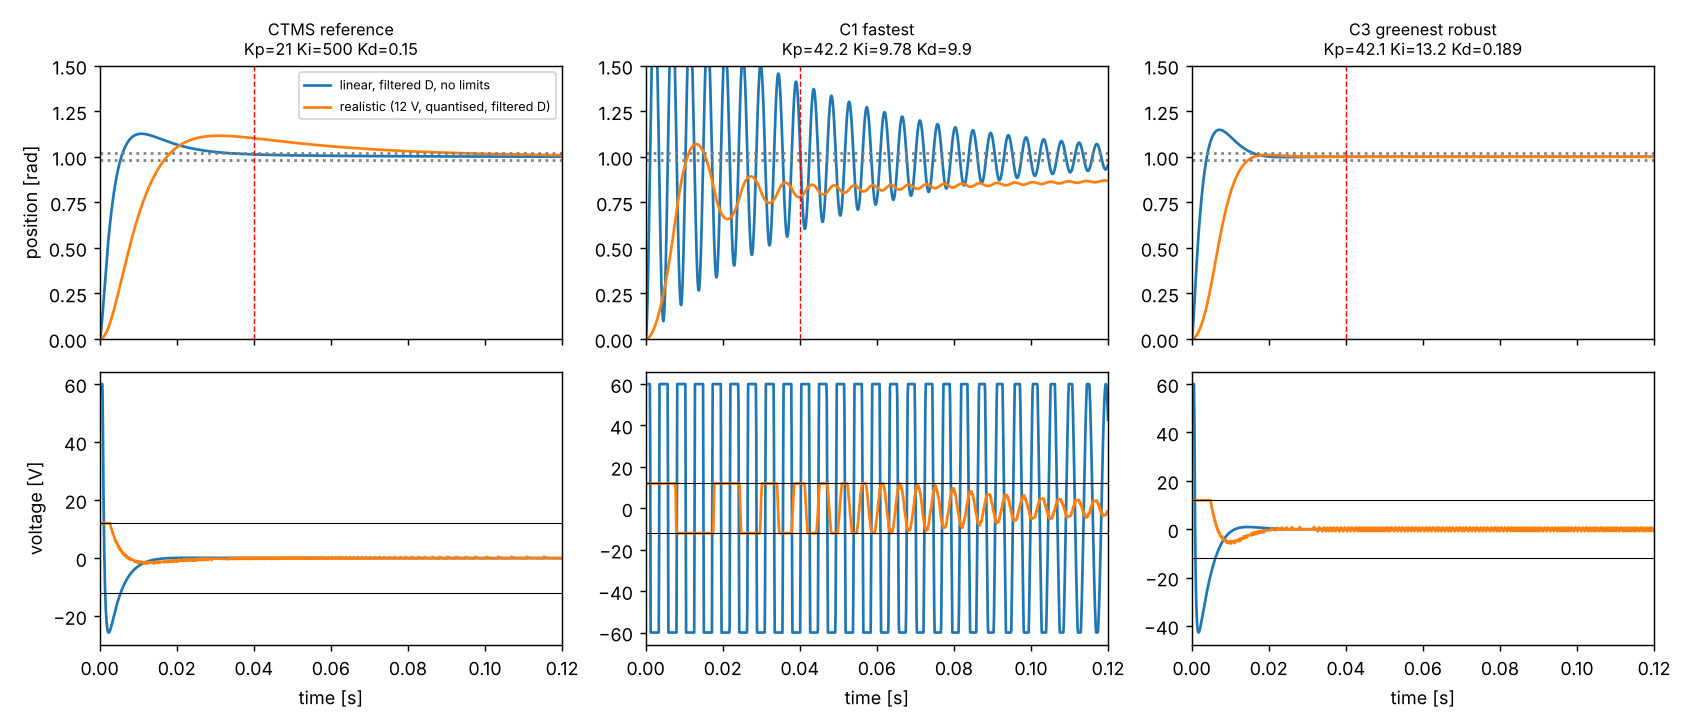
\includegraphics[width=0.98\textwidth]{case_study_dc_motor.png}
‫\end{center}
‫شکل: پاسخ پله و ولتاژ سه طرح؛ آبی بدون محدودیت (خطی با مشتق فیلترشده)، نارنجی واقع‌گرایانه (\lr{12 V}، کوانتیزه، مشتق فیلترشده). خط قرمز: ۰٫۰۴ ثانیه.
‫
‫\subsection{محدودیت‌ها}
‫یک موتور، یک مجموعه فرض، یک پلهٔ مرجع؛ بدون داده یا سخت‌افزار واقعی، بدون گشتاور بار، اصطکاک کولن و بک‌لش، بدون نوفهٔ حسگر فراتر از کوانتیزه‌سازی و بدون طراحی گسستهٔ خود کنترلر؛ بودجهٔ \lr{NSGA-II} کوچک (جمعیت ۲۰، ۱۵ نسل، ۳ بذر)؛ قاعدهٔ \lr{C3m} پس از دیدن نتایج افزوده شد؛ و این مطالعه \lr{LLM} را نمی‌آزماید (پارت ۷ هنوز منتظر اجرای زندهٔ مدل است).
‫
‫\subsection{پیامد برای \lr{agent} (ورودی پارت ۱۰)}
‫\lr{Agent} نباید فقط با حکم حلقهٔ آرمانی طرحی را «شدنی» گزارش کند. بررسی واقع‌گرایانه (محدودیت عملگر، ساختار و فیلتر مشتق، مونت‌کارلوی ناسازگاری) باید جزو گام راستی‌آزمایی شود و طرح‌هایی که ولتاژ آرمانی‌شان بسیار از حد عملگر بیشتر است باید علامت بخورند. اعداد خام: \texttt{\seqsplit{case\_study\_dc\_motor.csv}}.
‫
‫
‫\section{پارت ۱۰: یکپارچه‌سازی نهایی}
‫
‫\subsection{آنچه در این پارت انجام شد}
‫این پارت آزمایش تازه‌ای روی سیستم تازه نیست؛ سه کار می‌کند (بخش ۲۴ نوت‌بوک):
‫\begin{enumerate}
‫\item \textbf{پیامد یافتهٔ پارت ۹ را در \lr{agent} وارد می‌کند.} ابزار \texttt{\seqsplit{select\_greenest\_design}} اکنون \texttt{\seqsplit{loop\_check}} برمی‌گرداند. بدون حد عملگر، نتیجه با برچسب «\textbf{فقط حکم حلقهٔ آرمانی}» می‌آید؛ با ورودی \texttt{\seqsplit{v\_max\_volts}} طرح دوباره با آن حد، مشتق فیلترشده (\lr{$N=20$})، ضد-انباشت و ناسازگاری \lr{$\pm20\%$} روی بهره و مقیاس زمانی شبیه‌سازی می‌شود. اگر رد شود، پاسخ \lr{agent} صریحاً می‌گوید طرح نباید «شدنی» تلقی شود. سه اجرای کامل \lr{agent} (موتور \lr{DC} با \lr{12 V}؛ همان موتور بدون حد؛ همان موتور با \lr{0.5 V}) این رفتار را نشان دادند و ممیزی اعداد هر سه را پذیرفت. ابزار عدد مرجع پارت ۹ را بازتولید می‌کند (مرجع \lr{CTMS}: اوج ورودی ۳۴۹، نشست ۰٫۰۹۴ ثانیه، ۰٪ نمونه‌های ناسازگاری).
‫\item \textbf{یک اشکال مسیریابی کشف و رفع شد:} سیستم‌های با دقیقاً یک انتگرال‌گیر و بقیهٔ قطب‌ها پایدار (سروهای معمول) از مسیر \lr{PID} به \lr{LQR}/\lr{MPC} هدایت می‌شدند، با آنکه پارت ۹ نشان داد جست‌وجوی \lr{NSGA-II} روی آن‌ها کار می‌کند. اکنون برچسب «\lr{PID} (جست‌وجوی \lr{NSGA-II}؛ \lr{ZN} قابل‌اجرا نیست)» می‌گیرند؛ نوسان‌گرها و سیستم‌های ناپایدار حلقه‌باز بدون تغییر ماندند.
‫\item \textbf{مهر بازتولیدپذیری و جدول ادعا/شاهد} (در چکیدهٔ ابتدای گزارش و بخش ۲۴.۴ نوت‌بوک) و فهرست کارهای باقی‌مانده.
‫\end{enumerate}
‫
‫\subsection{محدودیت‌های این پارت}
‫\begin{itemize}
‫\item دروازهٔ جدید \textbf{فقط یک بررسی پس از انتخاب} است؛ جست‌وجو هنوز با شبیه‌ساز آرمانی انجام می‌شود و ممکن است طرح‌هایی پیشنهاد دهد که بعد رد می‌شوند.
‫\item ناسازگاری فقط بهره و مقیاس زمانی است (نه هر پارامتر فیزیکی جدا)؛ کوانتیزه‌سازی حسگر و اصطکاک کولن در این ابزار عمومی نیست (در پارت ۹ فقط کوانتیزه‌سازی بود).
‫\item آزمون دروازه روی یک گیاه واقعی (موتور \lr{DC}) و یک گیاه درسی انجام شد؛ این اثبات کلی بودن نیست.
‫\item دستور سامانهٔ افزوده‌شده در این پارت روی \lr{LLM} واقعی \textbf{آزموده نشد}؛ اجرای پارت ۷ پیش از آن و بدون آن انجام شد و نشان داد مدل‌های تا ۱۴ میلیارد پارامتر گاهی عدد بی‌منشأ می‌گویند، پس از تحلیل سیستم متوقف می‌شوند یا برای سامانهٔ خارج از محدوده طراحی می‌خواهند.
‫\end{itemize}
‫
‫\subsection{کارهای باقی‌مانده (به ترتیب اهمیت)}
‫\begin{enumerate}
‫\item تکمیل ارزیابی \lr{LLM} (بخش ۲۱.۶): تصمیم دربارهٔ نمره‌دادن به \lr{qwen3:14b} با سقف نشانه یا بدون تفکر (انحراف اعلام‌شده)، ثبت خطای هر مورد، برچسب‌زدن تکرارها در خروجی و ذخیرهٔ متن پاسخ‌ها، سپس اعمال دوبارهٔ قاعدهٔ ثبت‌شده بدون تغییر.
‫\item یک نمونهٔ \textbf{اندازه‌گیری‌شده} (پاسخ پلهٔ واقعی، حد منبع، تفکیک انکودر) به‌جای پارامترهای منتشرشده و فرض‌های ما.
‫\item وارد کردن شبیه‌ساز واقع‌گرایانه به خود جست‌وجو.
‫\item \lr{MIMO}، غیرخطی و طراحی گسسته همچنان خارج از محدوده‌اند.
‫\end{enumerate}
‫
‫
‫\section{وضعیت فعلی}
‫\begin{center}
‫\small
‫\begin{tabular}{|c|p{4.6cm}|p{5.6cm}|}
‫\hline
‫پارت & موضوع & وضعیت \\ \hline
‫۱ تا ۶ & مسئله، معماری، پیاده‌سازی \lr{agent}، منشأ معیارها، محک، ارزیابی مقایسه‌ای & انجام و اجرا شد \\ \hline
‫۷ & انتخاب \lr{LLM} متن‌باز & مهار و قاعده آماده؛ \textbf{هیچ مدل واقعی اجرا نشده} (منتظر اجرای زنده روی سامانهٔ نگارندگان) \\ \hline
‫۸ & نقشهٔ کاربردپذیری & انجام شد (۳۱ نقطه، ۳ بذر) \\ \hline
‫۹ & مطالعهٔ موردی موتور \lr{DC} & انجام شد؛ با پارامترهای منتشرشده، بدون سخت‌افزار \\ \hline
‫۱۰ & یکپارچه‌سازی نهایی & انجام شد (دروازهٔ بررسی واقع‌گرایانه، چکیده، جدول ادعا/شاهد) \\ \hline
‫\end{tabular}
‫\end{center}
‫نوت‌بوک (بخش‌های ۱ تا ۲۴) در محیط ساخت با \lr{Python}، \lr{python-control}، \lr{pymoo}، \lr{NumPy} و \lr{SciPy} واقعی به‌طور سرتاسری و بدون خطا اجرا شده است (نسخه‌ها در بخش ۲۴.۳ چاپ می‌شوند؛ زمان اجرا حدود ۳۰ دقیقه). گزارش \lr{LaTeX} فارسی در آن محیط \textbf{کامپایل نشده} است (فقط تعادل محیط‌ها و آکولادها بررسی شد)؛ پیش از تحویل باید با \lr{XeLaTeX} روی سامانهٔ نگارندگان کامپایل شود. محور پروژه همچنان طراحی یک دستیار برای مهندسی کنترل است که میان کیفیت کنترلی، استحکام و شاخص محیط‌زیستی تعادل برقرار می‌کند، با این تأکید که شاخص محیط‌زیستی نسبی است و حکم حلقهٔ آرمانی بدون بررسی واقع‌گرایانه کافی نیست.
‫
‫
‫\section*{منابع}
‫\addcontentsline{toc}{section}{منابع}
‫فهرست زیر منابعی است که در طول توسعهٔ پروژه (تمام مراحل، از جست‌وجوی
‫اولیهٔ اینترنتی تا آخرین مرحله) بررسی و مورد استفاده قرار گرفته‌اند.
‫عناوین به زبان اصلی (انگلیسی) آورده شده‌اند و پیوند مستقیم هرکدام نیز
‫ذکر شده تا امکان مراجعهٔ مجدد وجود داشته باشد.
‫
‫\begin{enumerate}
‫\item \lr{Guo, X. et al., ``ControlAgent: Automating Control System
‫Design via Novel Integration of LLM Agents and Domain Expertise'',
‫arXiv:2410.19811.}\\
‫\url{https://arxiv.org/abs/2410.19811}
‫
‫\item \lr{``AgenticControl: An Automated Control Design Framework Using
‫Large Language Models'', arXiv:2506.19160.}\\
‫\url{https://arxiv.org/abs/2506.19160}
‫
‫\item \lr{``SmartControl: Interactive PID controller design powered by
‫LLM agents and control system expertise'', ScienceDirect.}\\
‫\url{https://www.sciencedirect.com/science/article/pii/S235271102500161X}
‫
‫\item \lr{``LLM-based PID controller optimization'' -- systematic
‫literature review identifying five categories of LLM-based control-design
‫tools (prompt engineering, interactive tools, multi-agent architectures,
‫hybrid methods, hardware-validated applications), ResearchGate.}\\
‫\url{https://www.researchgate.net/publication/394118454_LLM-based_PID_controller_optimization}
‫
‫\item \lr{``Energy Modeling and Model Predictive Control for HVAC in
‫Buildings: A Review of Current Research Trends'', \emph{Energies}
‫15(19):7231, 2022.}\\
‫\url{https://doi.org/10.3390/en15197231}
‫
‫\item \lr{``LSTM-MPC Speed Prediction-Based DDQN Energy Management for
‫Hybrid Electric Vehicles'' -- objective function combining energy cost,
‫battery degradation cost, and equivalent social cost of carbon emissions,
‫PMC.}\\
‫\url{https://pmc.ncbi.nlm.nih.gov/articles/PMC12074296/}
‫
‫\item \lr{``Assessment of Product Carbon Footprint Reduction Potential
‫Using Lightweight Rotor Components for Electric Traction Motors'' --
‫permanent magnets responsible for 54\% of rotor-production emissions,
‫Springer (GCSM 2024).}\\
‫\url{https://link.springer.com/chapter/10.1007/978-3-031-93891-7_11}
‫
‫\item \lr{``Environmental impacts of electric motor technologies:
‫Life cycle approach based on EuP Eco-Report'' -- rare-earth magnet
‫mining/recycling environmental and supply-risk concerns, ScienceDirect.}\\
‫\url{https://www.sciencedirect.com/science/article/abs/pii/S0195925524003287}
‫
‫\item \lr{Kuru, H., ``A Carbon Footprint Study of Electric Motor
‫Production'' -- master's thesis providing the per-material emission
‫factors used in this project (magnets \textasciitilde 60 kg CO2e/kg,
‫steel \textasciitilde 27, aluminum \textasciitilde 2.07 primary /
‫\textasciitilde 0.61 recycled, copper \textasciitilde 3.5), Lappeenranta
‫University of Technology (LUT).}\\
‫\url{https://lutpub.lut.fi/bitstream/handle/10024/167611/mastersthesis_kuru_hanna.pdf}
‫
‫\item \lr{OSHA, ``Occupational Noise Exposure -- Overview'' -- official
‫85 dB(A) 8-hour action level and 90 dB(A) permissible exposure limit
‫(29 CFR 1910.95).}\\
‫\url{https://www.osha.gov/noise}
‫
‫\item \lr{Dou, Y. and Prempain, E., ``Green ILC: A Novel Energy-Efficient
‫Iterative Learning Control Approach'', \emph{Sensors} 24(23):7787, 2024.}\\
‫\url{https://pmc.ncbi.nlm.nih.gov/articles/PMC11644840/}
‫
‫\item \lr{National Renewable Energy Laboratory (NREL), ``Consumptive
‫Water Use for U.S. Power Production'' -- source of this project's default
‫water-intensity factor (1.8 L/kWh for thermoelectric generation).}\\
‫\url{https://docs.nrel.gov/docs/fy04osti/33905.pdf}
‫
‫\item \lr{U.S. Energy Information Administration (EIA), ``U.S. electric
‫power sector's use of water continued its downward trend in 2020'' --
‫national average water-intensity figures for comparison.}\\
‫\url{https://www.eia.gov/todayinenergy/detail.php?id=50698}
‫
‫\item \lr{Google, ``Measuring the environmental impact of AI inference''
‫(technical methodology report) and coverage thereof -- median Gemini
‫text-query figures of 0.24 Wh, 0.03 gCO2e, 0.26 mL water; source for
‫this project's data-center-overhead / full-stack accounting approach,
‫Data Center Dynamics.}\\
‫\url{https://www.datacenterdynamics.com/en/news/google-median-gemini-prompt-uses-024-watt-hours-of-power-and-consumes-026ml-of-water/}
‫
‫\item \lr{OpenAI (S. Altman) per-query energy figure (\textasciitilde 0.34
‫Wh per average ChatGPT query) and Epoch AI's independent corroborating
‫estimate, as compiled in Offset AI's methodology page.}\\
‫\url{https://www.offsetai.app/methodology-transparency-calculations}
‫
‫\item \lr{Ritchie, H., ``How much electricity does AI consume?'' -- IEA
‫methodology modeling agentic AI tasks as 4-6 sequential LLM calls,
‫Sustainability by Numbers (Substack).}\\
‫\url{https://hannahritchie.substack.com/p/ai-electricity-2025}
‫
‫\item \lr{Classical and H-infinity robustness theory (peak sensitivity
‫$M_s = \max_\omega|S(j\omega)|$, $S=1/(1+L)$) as covered in standard
‫control-theory references such as Åström, K. J. and Murray, R. M.,
‫\emph{Feedback Systems: An Introduction for Scientists and Engineers}
‫(freely available course text, Caltech/Lund).}\\
‫\url{https://www.cds.caltech.edu/~murray/amwiki/index.php/Feedback_Systems:_An_Introduction_for_Scientists_and_Engineers}
‫
‫\item \lr{Schick, T. et al., ``Toolformer: Language Models Can Teach Themselves to Use Tools'', arXiv:2302.04761, 2023.}\\
‫\url{https://arxiv.org/abs/2302.04761}
‫
‫\item \lr{Gao, L. et al., ``PAL: Program-aided Language Models'', arXiv:2211.10435, 2022.}\\
‫\url{https://arxiv.org/abs/2211.10435}
‫
‫\item \lr{Yao, S. et al., ``ReAct: Synergizing Reasoning and Acting in Language Models'', arXiv:2210.03629, 2022.}\\
‫\url{https://arxiv.org/abs/2210.03629}
‫
‫\item \lr{OpenAI, ``Function calling'' guide (the tool-calling schema format used by \texttt{OpenAICompatibleBackend}).}\\
‫\url{https://platform.openai.com/docs/guides/function-calling}
‫
‫\item \lr{Ollama, ``OpenAI compatibility'' documentation (serving open-weight models such as Qwen/Llama/Mistral behind the same API).}\\
‫\url{https://github.com/ollama/ollama/blob/main/docs/openai.md}
‫
‫\item \lr{Ollama model library pages (read 2026-10-12; sizes, context, tool support, license): Qwen3, Qwen3.6, Llama 3.1, Mistral Small 3.2, Ministral 3.}\\
‫\url{https://ollama.com/library/qwen3} \quad \url{https://ollama.com/library/qwen3.6} \quad \url{https://ollama.com/library/llama3.1} \quad \url{https://ollama.com/library/mistral-small3.2} \quad \url{https://ollama.com/library/ministral-3}
‫
‫\item \lr{Ollama, models with tool-calling support (search filter).}\\
‫\url{https://ollama.com/search?c=tools}
‫
‫\item \lr{Ollama Linux install script (used on Colab for the Part 7 live run; Ollama version not recorded).}\\
‫\url{https://ollama.com/install.sh}
‫
‫\item \lr{Google Colab, frequently asked questions: usage limits (free-tier GPU quota; on 14 Oct no GPU was available for several hours, which delayed the \texttt{llama3.1:8b} re-run to 15 Oct).}\\
‫\url{https://research.google.com/colaboratory/faq.html\#usage-limits}
‫
‫\item \lr{Åström, K. J. and Hägglund, T., ``Benchmark systems for PID control'', in \emph{Digital Control: Past, Present and Future of PID Control} (PID'00), Elsevier, 2000.}\\
‫\url{https://lup.lub.lu.se/record/537934}
‫
‫\item \lr{Control Tutorials for MATLAB and Simulink (CTMS, University of Michigan), ``DC Motor Position: System Modeling'' -- $P(s)=K/(s((Js+b)(Ls+R)+K^2))$.}\\
‫\url{https://ctms.engin.umich.edu/CTMS/index.php?example=MotorPosition&section=SystemModeling}
‫
‫\item \lr{Control Tutorials for MATLAB and Simulink (CTMS), ``DC Motor Position: PID Controller Design'' -- requirements (settling $<0.04$ s, overshoot $<16\%$) and the reference PID $K_p=21$, $K_i=500$, $K_d=0.15$ (read 2026-10-12).}\\
‫\url{https://ctms.engin.umich.edu/CTMS/index.php?example=MotorPosition&section=ControlPID}
‫
‫\item \lr{Deb, K., Pratap, A., Agarwal, S. and Meyarivan, T., ``A fast and elitist multiobjective genetic algorithm: NSGA-II'', \emph{IEEE Transactions on Evolutionary Computation} 6(2), 182--197, 2002.}\\
‫\url{https://doi.org/10.1109/4235.996017}
‫
‫\item \lr{Blank, J. and Deb, K., ``pymoo: Multi-Objective Optimization in Python'', \emph{IEEE Access} 8, 89497--89509, 2020.}\\
‫\url{https://doi.org/10.1109/ACCESS.2020.2990567} \quad \url{https://pymoo.org}
‫
‫\item \lr{Fuller, S., Greiner, B., Moore, J., Murray, R., van Paassen, R. and Yorke, R., ``The Python Control Systems Library (python-control)'', \emph{60th IEEE Conference on Decision and Control}, 2021.}\\
‫\url{https://python-control.org}
‫
‫\item \lr{Virtanen, P. et al., ``SciPy 1.0: fundamental algorithms for scientific computing in Python'', \emph{Nature Methods} 17, 261--272, 2020.}\\
‫\url{https://doi.org/10.1038/s41592-019-0686-2}
‫
‫\item \lr{Ziegler, J. G. and Nichols, N. B., ``Optimum settings for automatic controllers'', \emph{Transactions of the ASME} 64, 759--768, 1942 (the reaction-curve tuning rule used as the classical baseline).}
‫
‫\item \lr{Standard LaTeX special-character handling (the \% comment
‫character in particular) -- not a literature source but a methodological
‫note: the auto-generated report's rationale text was found, via actual
‫\texttt{pdflatex} compilation rather than syntax checking alone, to
‫truncate silently around unescaped \% characters; documented here as the
‫concrete reason this project now compiles its generated LaTeX output as
‫part of verifying each development stage, not just checks Python syntax.}
‫\end{enumerate}
‫
‫
‫\end{document}